% ===================================================================
%  LaTeX source for:
%  "Long-term Performance Assessment of a Radiological Laboratory in
%   IAEA Proficiency Tests (2021-2025): A Multi-dimensional Analysis"
%
%  Compiled with:  pdflatex main && pdflatex main && pdflatex main
% ===================================================================
\documentclass[12pt,a4paper,twoside]{article}

% ---------- Packages ----------
\usepackage[utf8]{inputenc}
\usepackage[T1]{fontenc}
\usepackage{mathptmx}            % Times-like font
\usepackage[scaled=0.92]{helvet} % sans-serif for headings
\usepackage{courier}
\usepackage{amsmath,amssymb}
\usepackage{graphicx}
\usepackage[labelfont=bf,font=small,skip=6pt]{caption}
\usepackage[labelfont=bf,font=small,skip=4pt]{subcaption}
\usepackage[margin=2.5cm,headheight=14pt]{geometry}
\usepackage{booktabs}
\usepackage{multirow}
\usepackage{array}
\usepackage{doi}
\usepackage{hyperref}
\usepackage[numbers,sort&compress]{natbib}
\usepackage{fancyhdr}
\usepackage{setspace}
\usepackage{enumitem}
\usepackage{float}
\usepackage{xcolor}
\usepackage{colortbl}

% ---------- Linespread (double / 1.5 spacing for submission) ----------
\onehalfspacing

% ---------- Hyperlinks ----------
\hypersetup{
  colorlinks=true,
  linkcolor=blue,
  citecolor=blue,
  urlcolor=blue
}

% ---------- Page headers / footers ----------
\pagestyle{fancy}
\fancyhf{}
\fancyhead[LE,RO]{\small \textit{IAEA Proficiency Test Performance Analysis (2021--2025)}}
\fancyhead[RE,LO]{\small \thepage}
\fancyfoot[CE,CO]{}
\renewcommand{\headrulewidth}{0.4pt}

% ---------- Title ----------
\title{\textbf{Long-term Performance Assessment of a Radiological Laboratory\\
in IAEA Proficiency Tests (2021--2025):\\
A Multi-dimensional Statistical Analysis}}

\author{%
  \large Yunlong Li$^{1,2,*}$, Jianfeng Lu$^{1,2}$ \\[4pt]
  \small $^1$ Radiation Monitoring Technical Center, Hangzhou, Zhejiang, China\\
  \small $^2$ Key Laboratory of Radiation Environmental Monitoring, \\ \small Ministry of Ecology and Environment, Hangzhou, Zhejiang, China\\
  \small $^*$ Corresponding author: yl-li15@tsinghua.org.cn
}
\date{}

% ===================================================================
\begin{document}

\maketitle

% ---------- Abstract ----------
\begin{abstract}
\noindent
This study presents a multi-dimensional framework for longitudinal proficiency test (PT) performance assessment, demonstrated through the analysis of one Chinese radiological laboratory's performance in five consecutive IAEA PT rounds (2021--2025), covering 135 measurements across 133 analyte--matrix combinations. Six analytical dimensions were evaluated: project difficulty coefficients, temporal difficulty trends, inter-laboratory ranking, difficulty-tier stratification, a weighted Result Deviation Index (RDI), and within-project relative bias ranking. The overall pass rate was 98.5\% (133/135 scored ``Acceptable''), with zero ``Not Acceptable'' results. The weighted RDI remained consistently below the all-laboratory mean (5-year mean 3.05\%, range 1.41\%--4.66\%). A Wilcoxon signed-rank test confirmed that the laboratory's absolute relative bias was significantly lower than the peer median across 109 project participations ($p < 0.001$). In the ``Hard'' difficulty tier, a 91.7\% (11/12) pass rate was maintained, substantially exceeding the global average for those projects. Although annual difficulty coefficients fluctuated (mean range 0.553--0.734), Mann--Kendall trend tests did not detect statistically significant temporal trends in difficulty, pass rate, or RDI at the $\alpha = 0.05$ level over the 5-year period. These results demonstrate the value of multi-dimensional PT performance assessment beyond the conventional pass/fail framework and provide a template for other laboratories seeking to extract richer insights from their PT data.

\vspace{6pt}
\noindent\textbf{Keywords:} IAEA proficiency test; radionuclide determination; laboratory performance; Result Deviation Index; difficulty coefficient; relative bias; quality assurance
\end{abstract}

% ===================================================================
\section{Introduction}
% ===================================================================

The International Atomic Energy Agency (IAEA) has organized annual proficiency tests (PTs) for the determination of radionuclides in environmental samples for over five decades~\cite{iaea1989,iaea2017}. Participating laboratories report measured activity concentrations ($x_{\text{rep}}$) and associated standard uncertainties ($u_{\text{rep}}$) for spiked test materials (water, soil, sediment, vegetation, or surface wipes). The IAEA evaluates each result against an assigned reference value ($x_{\text{ref}}$) with standard uncertainty ($u_{\text{ref}}$) using a two-component assessment framework based on ISO 13528:2022~\cite{iso13528}:

\textbf{Trueness assessment.} The relative bias is calculated as $\text{RB} = (x_{\text{rep}} - x_{\text{ref}}) / x_{\text{ref}} \times 100\%$. If $|\text{RB}| \leq \text{MARB}$, where MARB is the Maximum Acceptable Relative Bias determined for each analyte considering the radioanalytical method, activity level, and matrix complexity, the result is rated ``Accepted'' for trueness~\cite{deregge2000}.

\textbf{Precision assessment.} The $P$ statistic evaluates whether the reported uncertainty adequately covers the observed bias: $P = \sqrt{ (u_{\text{ref}}/x_{\text{ref}})^2 + (u_{\text{rep}}/x_{\text{rep}})^2 } \times 100\%$. The precision rating is ``Accepted'' when \emph{both} $|\text{RB}| \leq k \cdot P$ (with coverage factor $k = 2.58$ for 99\% confidence) and $P \leq \text{MARB}$ are satisfied. If either condition fails, precision is rated ``Not Accepted''.

\textbf{Final score.} The combined final score is: ``Acceptable'' (A) when both trueness and precision are Accepted; ``Warning'' (W) when trueness is Accepted but precision is Not Accepted; and ``Not Acceptable'' (N) when trueness is Not Accepted.

\textbf{Z-score.} For intercomparison purposes, a Z-score is computed as $Z = (x_{\text{rep}} - x_{\text{ref}}) / \sigma_{\text{PT}}$, where the standard deviation for proficiency assessment is $\sigma_{\text{PT}} = (\text{MARB} \cdot x_{\text{ref}}) / 3$~\cite{iso13528}. For parameters without independently assigned target values (gross $\alpha$/$\beta$ measurements), a consensus-value approach is used with robust statistics.

For the IAEA PT rounds analyzed in this study, most projects had independently assigned target values by formulation or characterization; only gross alpha/beta measurements used the consensus approach. Where only a Z-score was reported (without an explicit final score), the conventional threshold $|Z| \leq 2 \Rightarrow$ A, $2 < |Z| < 3 \Rightarrow$ W, $|Z| \geq 3 \Rightarrow$ N was applied.

While the per-project pass/fail outcome serves accreditation purposes, it provides only a one-dimensional snapshot. A consistently ``A''-scoring laboratory may still exhibit systematic biases or struggle with certain analyte--matrix pairs~\cite{siddique2012,cujic2019}. Moreover, project difficulty varies considerably across rounds, nuclides, and matrices. A meaningful long-term assessment requires a framework that simultaneously considers accuracy, consistency, and relative standing among peer laboratories.

Since 2021, our laboratory has participated in all five IAEA TERC PT rounds (2021--2025)~\cite{iaea2021report,iaea2022report,iaea2023report,iaea2024report,iaea2025report}, completing 135 measurements across 133 project types. This study applies six complementary analytical dimensions to these data: (1) project difficulty coefficients and pass rates, (2) how difficulty has changed over time, (3) inter-laboratory ranking by participation and A-score counts, (4) performance by difficulty tier, (5) the Result Deviation Index (RDI), and (6) within-project ranking by relative bias~\cite{karfopoulos2025}.

% ===================================================================
\section{Materials and Methods}
% ===================================================================

\subsection{IAEA Proficiency Test Program (2021--2025)}

Each year, 28--56 spiked test items (``projects'') were distributed, covering gamma, beta, and alpha emitters in water, soil, sediment, vegetation, and surface-wipe matrices~\cite{hou2008}. Table~\ref{tab:yearly_overview} summarizes each round.

\begin{table}[H]
\centering
\caption{Overview of IAEA TERC proficiency test rounds analyzed in this study.}
\label{tab:yearly_overview}
\resizebox{\linewidth}{!}{
\begin{tabular}{@{}lcccccc@{}}
\toprule
\textbf{Year} & \textbf{PT Identifier} & \textbf{No.\ Projects} & \textbf{No.\ Labs} & \textbf{Mean Difficulty} & \textbf{Median Difficulty} & \textbf{Max Difficulty} \\
\midrule
2021 & TEL-2021-03  & 28  & 270 & 0.553 & 0.626 & 0.944 \\
2022 & TERC-2022-01 & 56  & 277 & 0.734 & 0.821 & 0.996 \\
2023 & TERC-2023-01 & 40  & 319 & 0.685 & 0.749 & 0.991 \\
2024 & TERC-2024-01 & 47  & 472 & 0.685 & 0.663 & 0.977 \\
2025 & TERC-2025-01 & 42  & 399 & 0.683 & 0.738 & 0.980 \\
\bottomrule
\end{tabular}
}
\par\vspace{4pt}\footnotesize Note: ``No.\ Labs'' refers to all distinct laboratories that participated in the PT round. RDI-related statistics (Table~\ref{tab:rdi_summary}) use a smaller denominator because some projects do not report relative bias values.
\end{table}


\subsection{Data Collection and Preprocessing}
The original data were provided by the IAEA in the form of annual summary reports~\cite{iaea2021report,iaea2022report,iaea2023report,iaea2024report,iaea2025report}. Each report is organized into separate data tables, with each table containing the results of all participating laboratories for a single PT project. Each project is identified by a combination of nuclide, decay mode, and matrix---for example, ``Cs-137 Gamma Water'' refers to the determination of Cs-137 activity by measuring its gamma emissions in a water matrix. For the small number of results where only a Z-score was provided without an explicit final score, the threshold $|Z| \leq 2 \Rightarrow$ A, $2 < |Z| < 3 \Rightarrow$ W, $|Z| \geq 3 \Rightarrow$ N was applied (see Section~1 for the relationship between Z-score and the evaluation framework). All data processing, statistical computation, and visualization code are available at: \href{https://github.com/yunlongli15/iaea-pt-analysis-2021-2025}{https://github.com/yunlongli15/iaea-pt-analysis-2021-2025}.

Our laboratory participated under different numerical codes in different years owing to IAEA's anonymized assignment scheme: Labcode~211 (2021), 8 (2022), 43 (2023), 5 (2024), and 15 (2025). The total number of projects in which our laboratory participated ranged from 12 (2021) to 35 (2025), reflecting an evolving scope of analytical capabilities.

\subsection{Performance Metrics}

\subsubsection{Difficulty Coefficient}

For each project $j$ in year $y$, the \textbf{difficulty coefficient} $D_{j,y}$ is defined as:
\begin{equation}
  D_{j,y} = 1 - \frac{N_{j,y}^{(A)}}{N_{y}^{\text{(all labs)}}}
  \label{eq:difficulty}
\end{equation}
where $N_{j,y}^{(A)}$ denotes the number of laboratories scoring ``A'' for that project and $N_{y}^{\text{(all labs)}}$ denotes the total number of distinct laboratories that participated in the PT round that year. The \textbf{pass rate} is defined as $P_{j,y} = N_{j,y}^{(A)} / N_{j,y}^{\text{(total)}}$, where $N_{j,y}^{\text{(total)}}$ is the number of laboratories that submitted results for that specific project. The two metrics use different denominators and are not complementary.

Projects are classified into four difficulty tiers: Very Easy ($D < 0.6$), Easy ($0.6 \leq D \leq 0.8$), Moderate ($0.8 < D \leq 0.9$), and Hard ($D > 0.9$)~\cite{iaea2017}.

\subsubsection{Result Deviation Index (RDI)}

For a given laboratory $i$ in year $y$, the (weighted) Result Deviation Index is defined as:
\begin{equation}
  \text{RDI}_{i,y} = \frac{1}{K} \sum_{k=1}^{K} w^{(k)}_y \cdot \bigl| \text{RB}_{i,y}^{(k)} \bigr|,
  \qquad w^{(k)}_y = \frac{1.2}{1 + \text{MARB}^{(k)}_y / 100\%}
  \label{eq:rdi}
\end{equation}
where $\text{RB}_{i,y}^{(k)}$ is the relative bias for project $k$ and $\text{MARB}^{(k)}_y$ is the Maximum Acceptable Relative Bias determined by the IAEA for that project. The MARB reflects the achievable precision given the radioanalytical method, activity level, and matrix complexity. The constant 1.2 normalizes the weight to unity at $\text{MARB} = 20\%$, which is the most common MARB value across IAEA PT projects: a project with $\text{MARB} = 20\%$ receives $w = 1.0$, while a project with $\text{MARB} = 50\%$ receives $w \approx 0.80$, preventing such projects from disproportionately inflating the RDI. For a small number of projects for which no MARB value was provided in the IAEA evaluation reports, a default weight of $w = 1.0$ (equivalent to $\text{MARB} = 20\%$) was assigned.

It should be noted that not all IAEA PT projects report a relative bias value; some provide only a reported value, reported uncertainty, and Z-score without disclosing the assigned (target) value. Such projects are necessarily excluded from all RDI calculations and RDI-based rankings. Consequently, the number of laboratories included in RDI-related statistics (Table~\ref{tab:rdi_summary}) is smaller than the total number of laboratories in the PT round (Table~\ref{tab:yearly_overview}), since laboratories that participated exclusively in projects without reported relative bias are absent from the RDI ranking pool.

\subsubsection{Relative Bias and Percentile Ranking}

Within each project, laboratories are ranked by their absolute relative bias $|\text{RB}|$ in ascending order: the laboratory with the smallest $|\text{RB}|$ (closest to the assigned value) ranks first. The percentile rank of our laboratory is then computed as $\text{Rank}/N_{\text{total}} \times 100\%$, where $N_{\text{total}}$ is the number of laboratories that submitted results for that project. A percentile of $x\%$ means that $x\%$ of participating laboratories achieved a smaller absolute relative bias than our laboratory — i.e., only $x\%$ of the cohort was more accurate. This within-project ranking controls for the varying intrinsic difficulty of different nuclide--matrix combinations, since each laboratory is compared only against others measuring the same analyte in the same matrix.

\subsection{Statistical Analysis}

All statistical analyses were performed using Python 3.11 with the \texttt{pandas} (2.0), \texttt{numpy} (1.24), \texttt{scipy} (1.11), and \texttt{matplotlib} (3.7) libraries. Box-and-whisker plots show the median (center line), interquartile range (IQR; box), and whiskers extending to the furthest data point within $1.5 \times \text{IQR}$ from the box.

Temporal trends in annual difficulty coefficients, pass rates, RDI values, and percentile ranks were assessed using the non-parametric Mann--Kendall trend test, which does not assume linearity or normality and is suitable for short time series ($N = 5$ years). Year-to-year differences in percentile rank distributions were tested with the Kruskal--Wallis one-way analysis of variance by ranks. A one-sample Wilcoxon signed-rank test (one-sided) was used to evaluate whether our laboratory's absolute relative bias was systematically lower than the all-laboratory median across projects. Wilson score intervals were computed for tier-aggregated pass rates. All tests used $\alpha = 0.05$ as the significance threshold. Trend lines in time-series plots are simple linear interpolations connecting annual means and are not intended to imply a parametric model.

% ===================================================================
\section{Results and Discussion}
% ===================================================================

\subsection{Overview of Project Difficulty and Pass Rates}
\label{sec:difficulty_overview}

Figure~\ref{fig:difficulty_overview} presents how project difficulty varied from 2021 to 2025. The mean difficulty coefficient, defined with respect to the total PT-round cohort, fluctuated between 0.553 (2021) and 0.734 (2022), then remained near 0.685 (2023--2025). The 2022 round had the highest mean and median difficulty (median $D = 0.821$, maximum 0.996), reflecting a large number of specialized projects with limited participation. A Mann--Kendall trend test over the five annual means did not detect a statistically significant monotonic trend ($S = -2$, $p = 0.81$), indicating that the year-to-year fluctuations are consistent with random variation at $\alpha = 0.05$. Similarly, while the mean pass rate declined from 86.6\% (2021) to 74.1\% (2025), this decline was not statistically significant ($S = -6$, $p = 0.22$). Given the small number of years ($N = 5$), statistical power to detect genuine trends is limited; the observed fluctuations should therefore be interpreted as descriptive patterns rather than confirmed trends.

\begin{figure}[H]
  \centering
  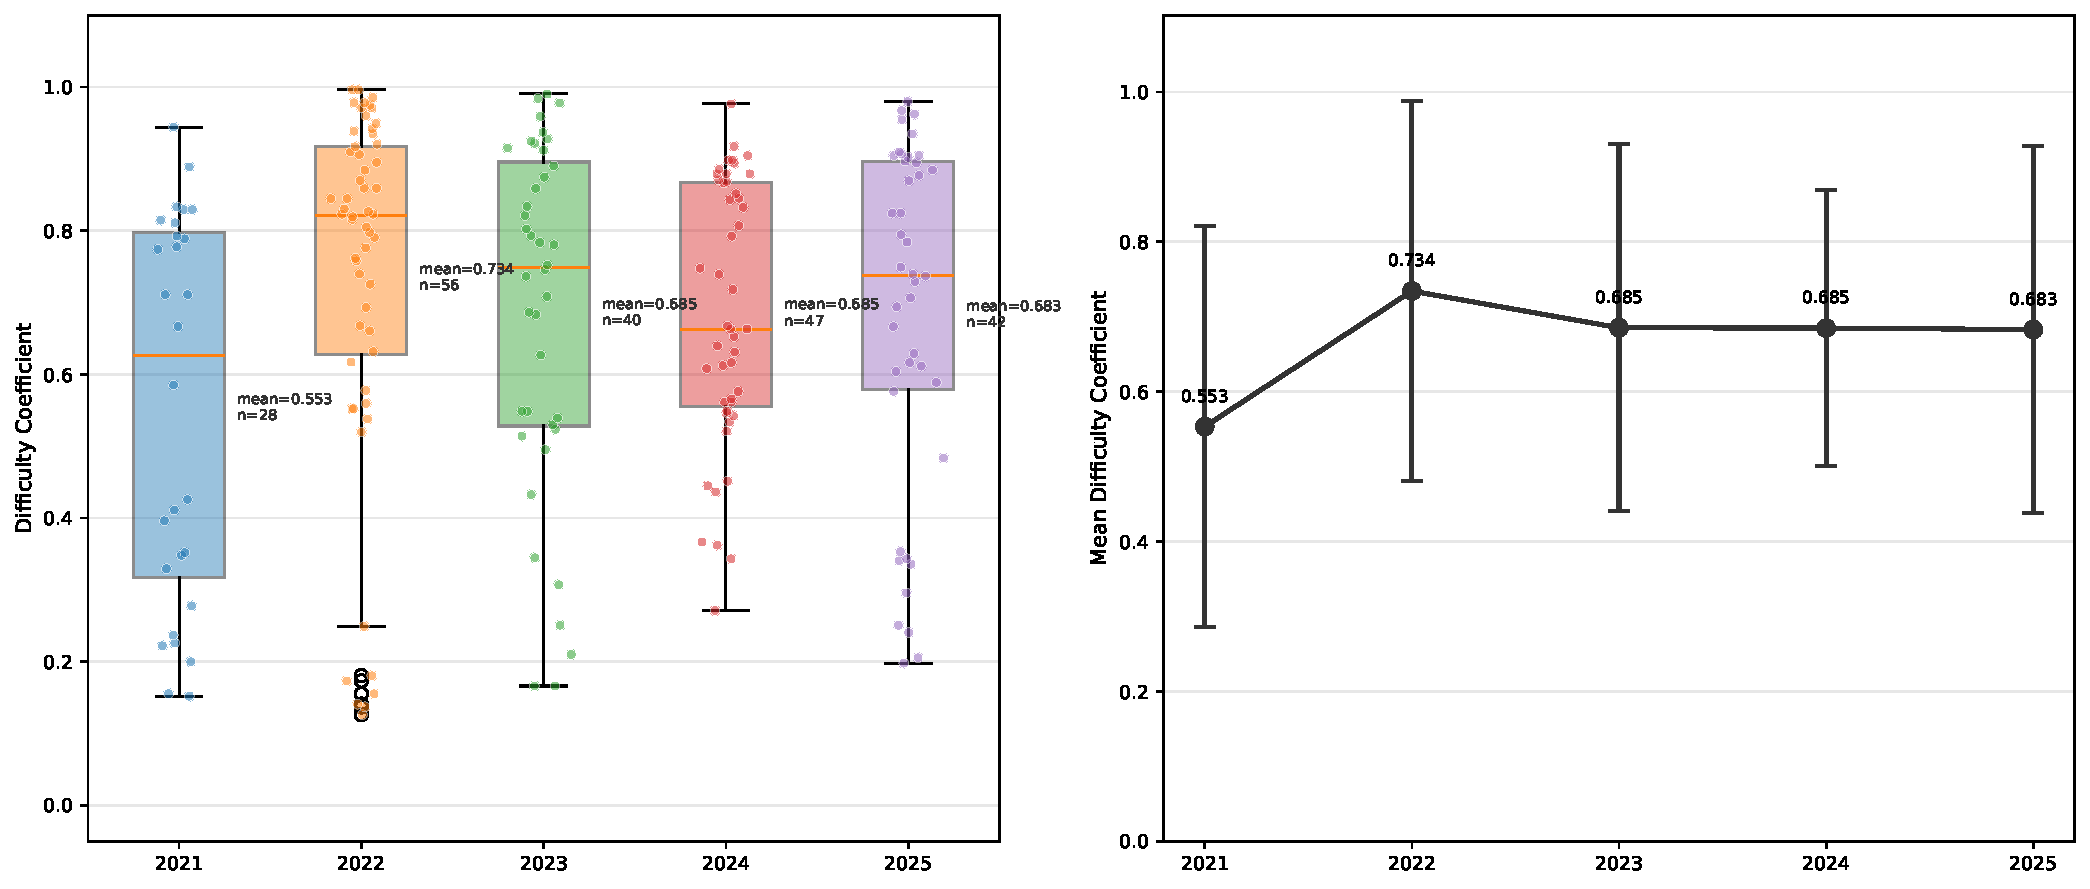
\includegraphics[width=0.98\textwidth]{figures/fig_difficulty_overview.pdf}
  \caption{(a) Distribution of project difficulty coefficients (boxplots) across the five years. The notches denote the 95\% confidence interval for the median. (b) Mean difficulty trend with $\pm 1$ standard deviation error bars.}
  \label{fig:difficulty_overview}
\end{figure}

Several factors may contribute to the observed inter-year variation in difficulty. The IAEA TERC has expanded the range of matrices and radionuclides offered, increasingly including challenging analytes such as $^{210}$Po (alpha spectrometry), $^{235}$U (ICP-MS and gamma spectrometry), and complex decay-chain nuclides in soil/sediment matrices. The participating laboratory pool has grown substantially (from 270 in 2021 to 472 in 2024), incorporating more laboratories with varying levels of experience, which could increase the observed variance and reduce the pass rate. Regardless of the cause, the magnitude of year-to-year difficulty variation underscores the importance of normalizing a laboratory's performance by the contemporaneous difficulty level when making inter-year comparisons.

Figure~\ref{fig:difficulty_2025} illustrates the 2025 round with individual project difficulty coefficients and pass rates. The hardest project was ``Pa-234m Gamma Soil'' ($D = 0.980$, pass rate 33.3\%), while ``Co-60 Gamma Water'' was the easiest ($D = 0.198$, pass rate 95.2\%). Gamma-emitting nuclides in water matrices consistently showed lower difficulty, whereas alpha emitters and uranium isotopes in soil matrices exhibited the highest difficulty coefficients.

\begin{figure}[H]
  \centering
  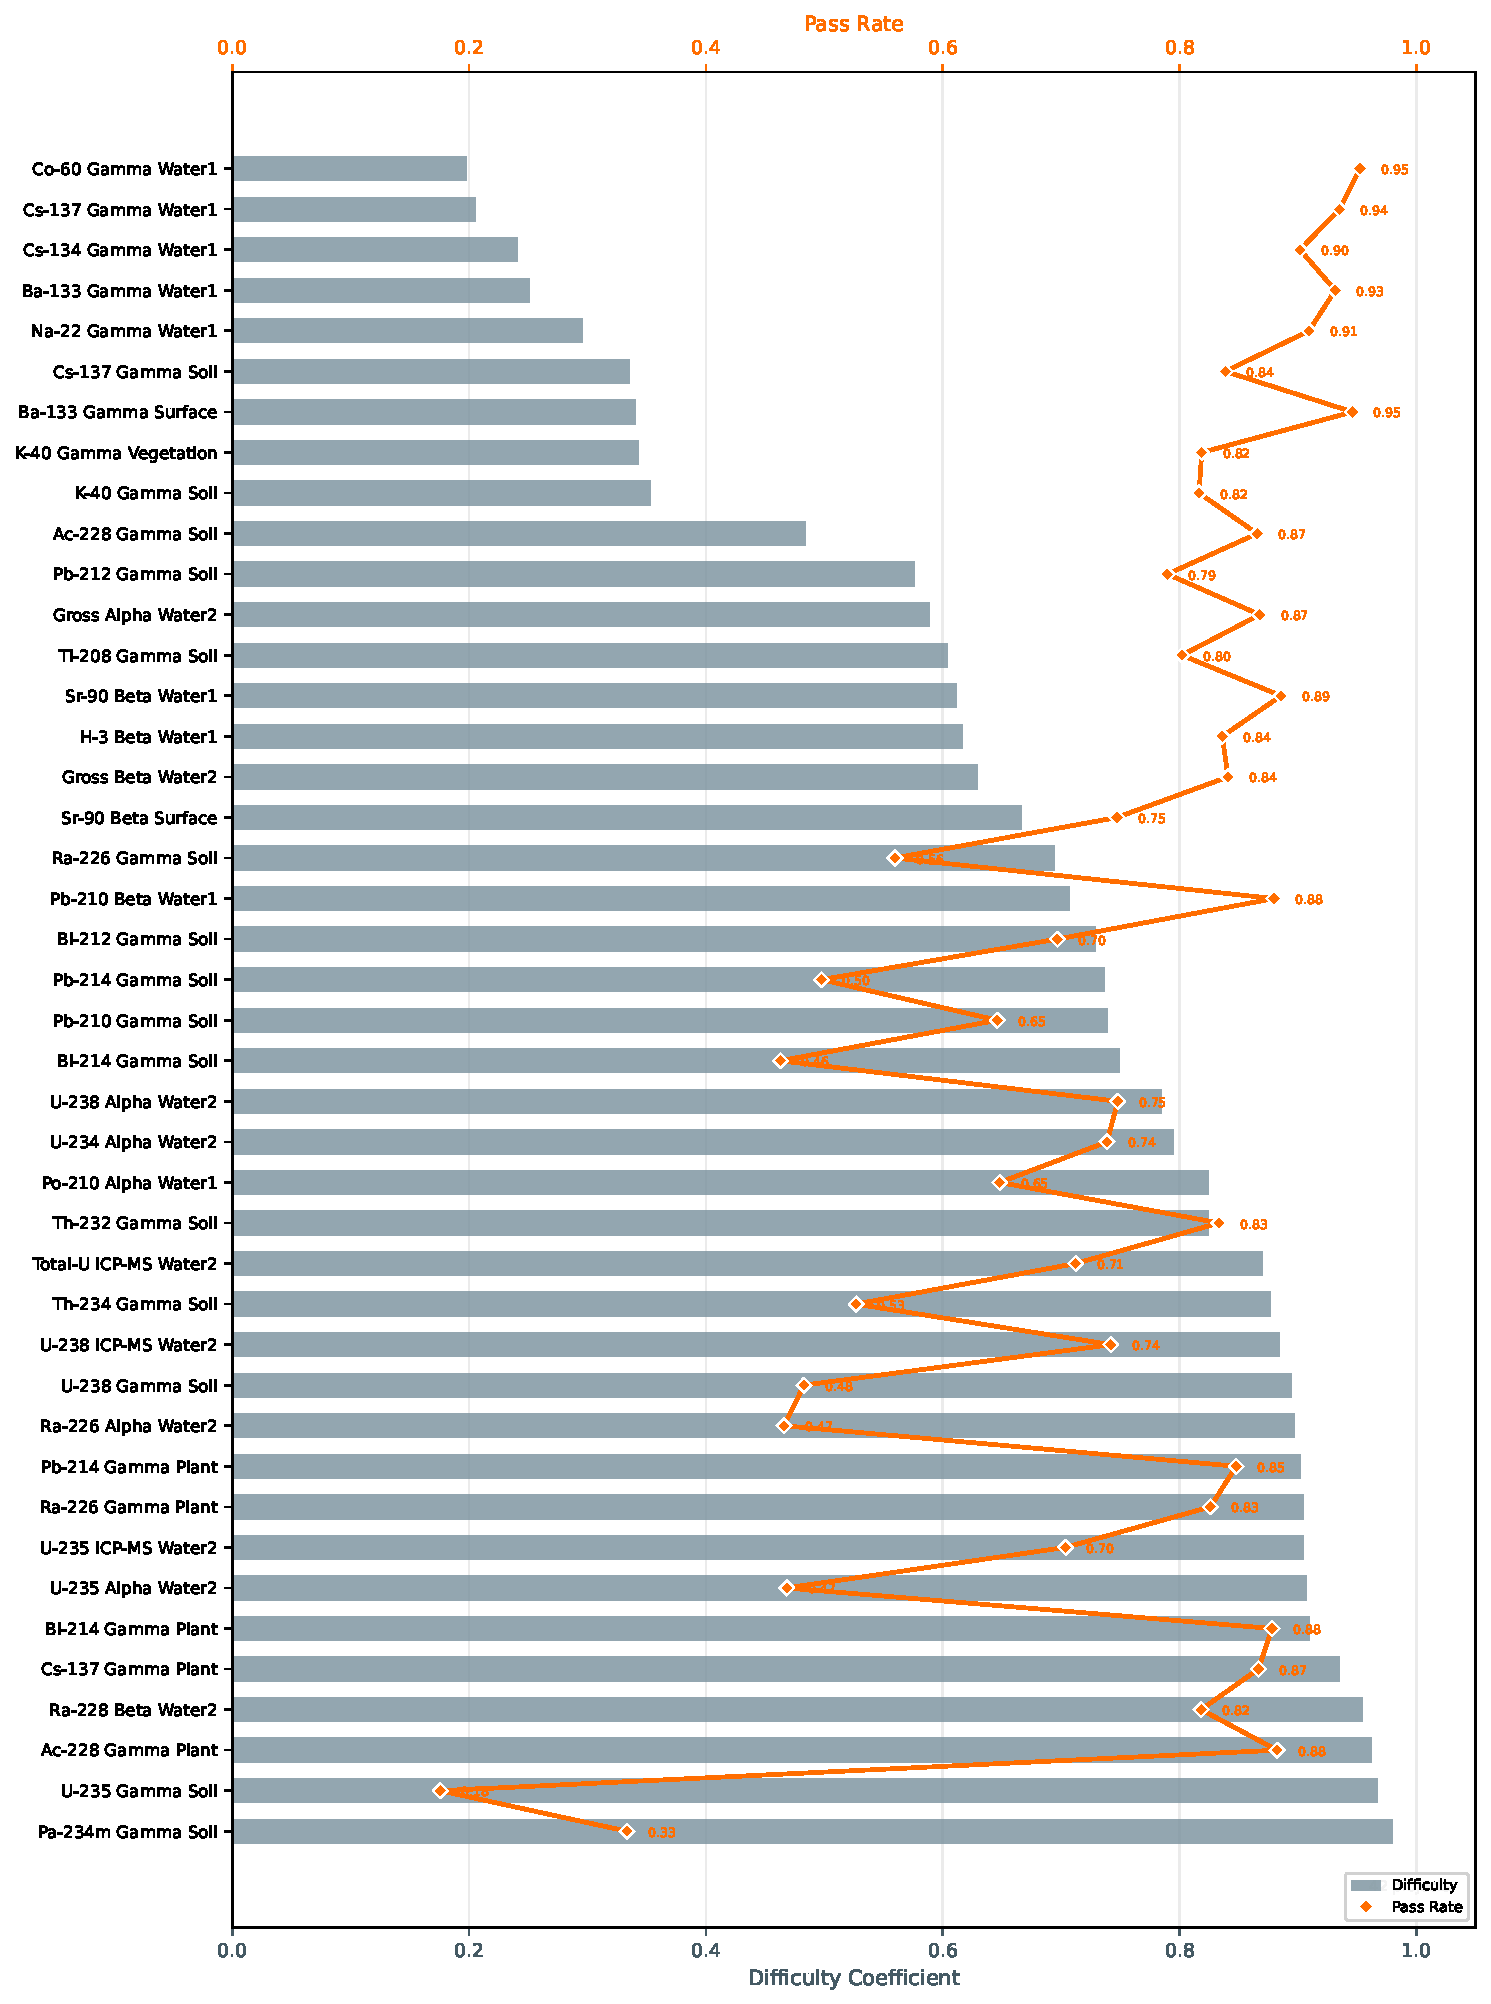
\includegraphics[width=0.98\textwidth]{figures/fig_difficulty_pass_rate_2025.pdf}
  \caption{Project difficulty coefficients (bars, bottom axis) and pass rates (diamond markers, top axis) for the 2025 IAEA TERC PT round. The two metrics use different denominators and are not complementary.}
  \label{fig:difficulty_2025}
\end{figure}

\subsection{Temporal Trends in Project Difficulty}
\label{sec:difficulty_trends}

To examine how the difficulty of specific radionuclide--matrix combinations has changed over time, we matched projects across years using their \texttt{project\_core} identifiers. When a project type appeared as multiple variants within the same year (e.g., Water1, Water2, Water3), the difficulties and pass rates of these variants were merged using a weighted average, with the number of participating laboratories in each variant serving as the weight. This analysis was restricted to project cores appearing in three or more years (i.e., at least three of the five rounds).

Figure~\ref{fig:difficulty_trends} highlights the eight projects with the largest difficulty increase and the eight with the largest decrease over the study period. The largest increase was ``Pb-210 Gamma Water,'' which rose from $D = 0.650$ to $D = 0.977$ ($\Delta D = +0.33$), followed by ``U-235 Gamma Soil'' ($\Delta D = +0.06$) and ``Pa-234m Gamma Soil'' ($\Delta D = +0.04$). Conversely, several projects showed substantial difficulty decreases: ``Ac-228 Gamma Soil'' dropped from $D = 0.762$ to $D = 0.484$ ($\Delta D = -0.28$), ``Cs-137 Soil'' from 0.823 to 0.561 ($\Delta D = -0.26$), and ``Pb-212 Gamma Soil'' from 0.820 to 0.576 ($\Delta D = -0.24$). 

\begin{figure}[H]
  \centering
  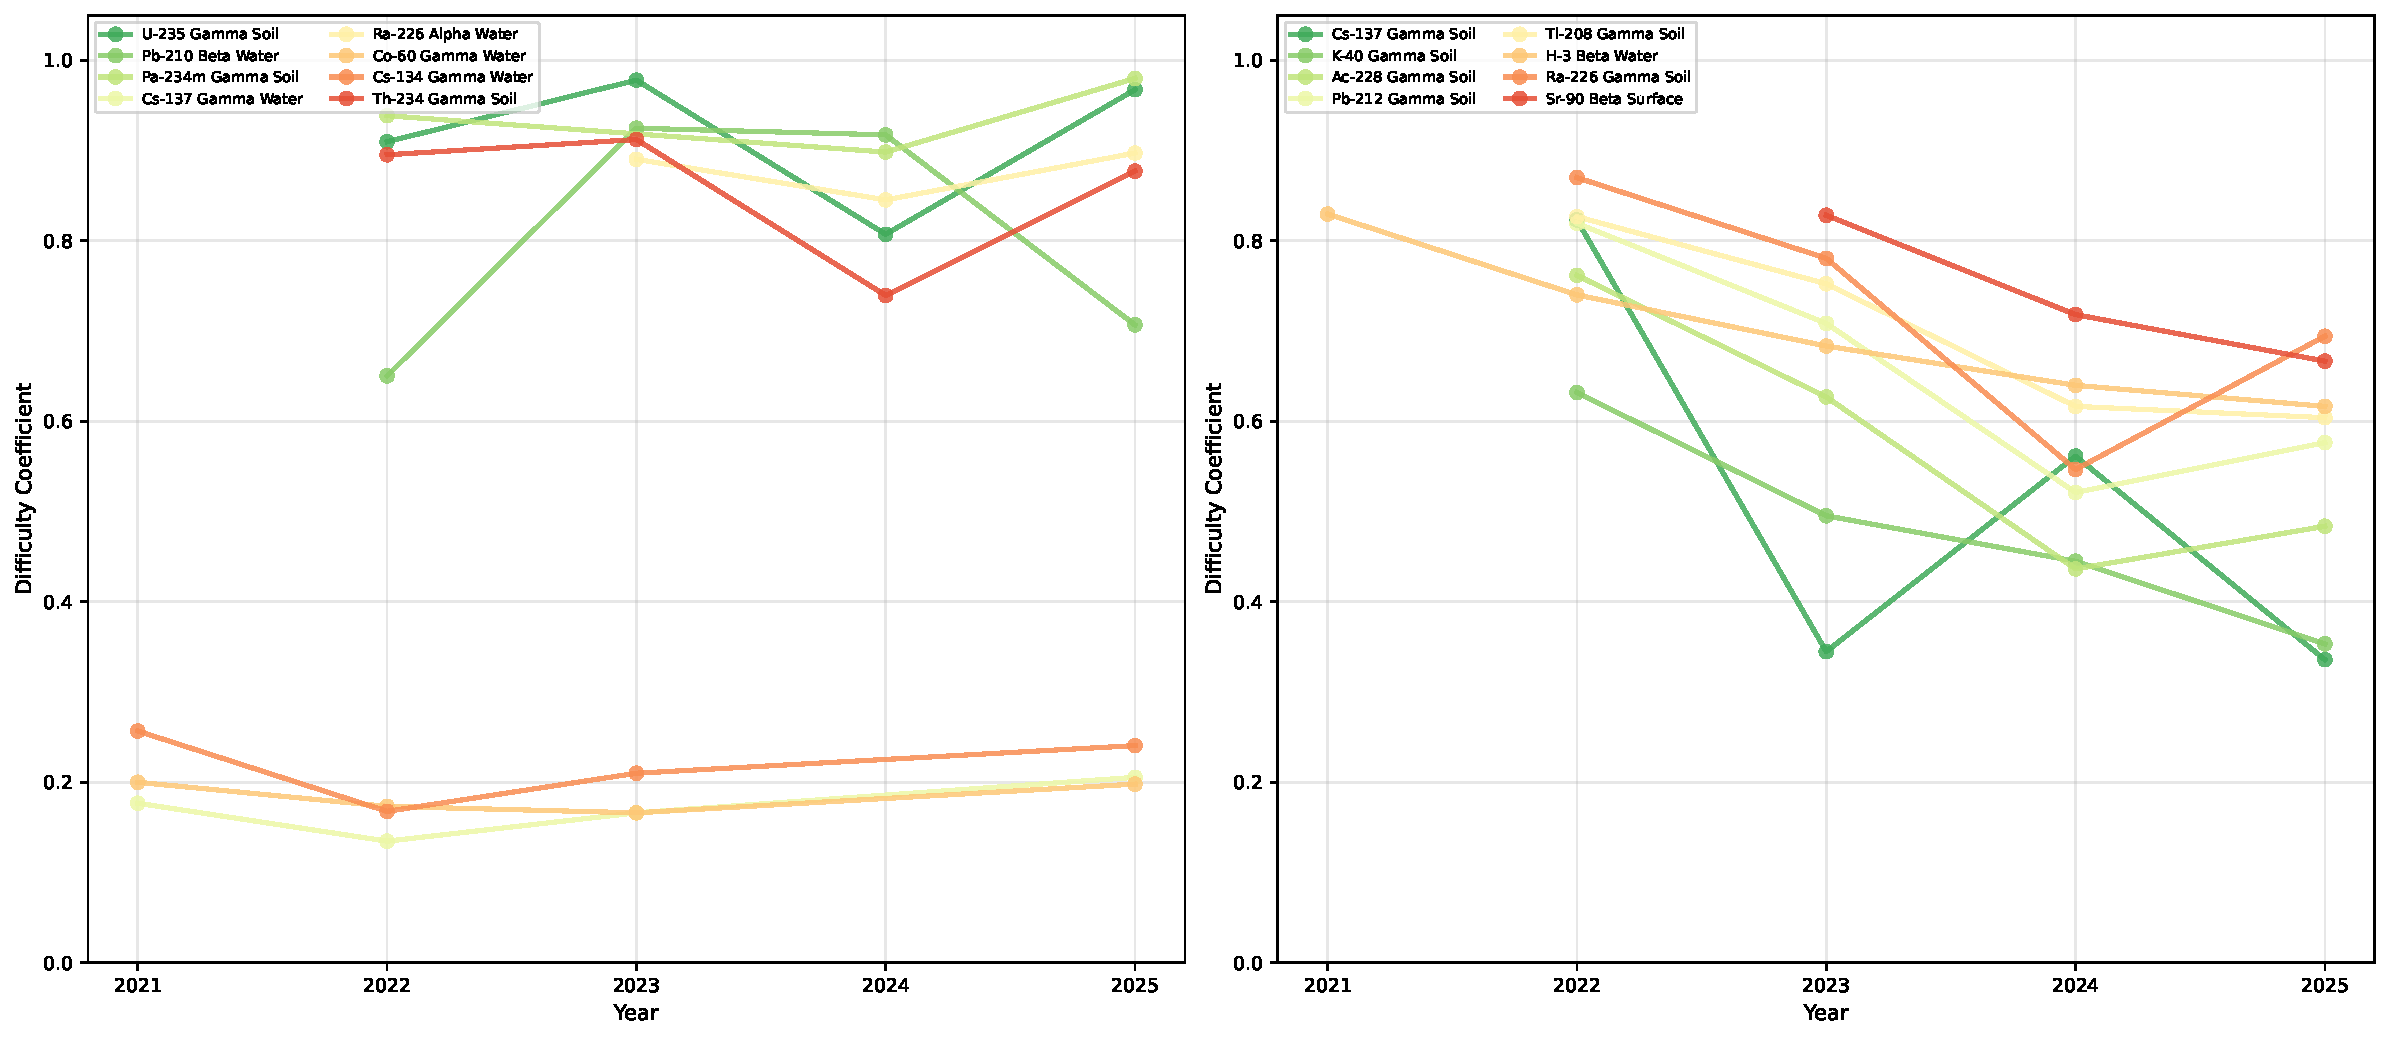
\includegraphics[width=0.98\textwidth]{figures/fig_difficulty_trends.pdf}
  \caption{Temporal trends in project difficulty for projects appearing in $\geq 3$ years. Left: eight projects with the largest difficulty increase. Right: eight projects with the largest decrease.}
  \label{fig:difficulty_trends}
\end{figure}

The heatmap in Figure~\ref{fig:difficulty_heatmap} provides a comprehensive overview of all multi-year projects. A gradient from green (easy, $D \approx 0$) to red (difficult, $D \approx 1$) reveals clusters of persistently easy projects (e.g., gamma emitters in water: Co-60, Cs-134, Cs-137) and persistently challenging ones (e.g., U-235, Pa-234m, Pb-210 in soil matrices). The heatmap also reveals year-to-year volatility for certain projects (e.g., ``Sr-90 Beta Surface'' was hard in 2021 but became moderate by 2024--2025), which may reflect changes in the spiked activity level, the sample matrix composition, or the participating laboratory cohort.

\begin{figure}[H]
  \centering
  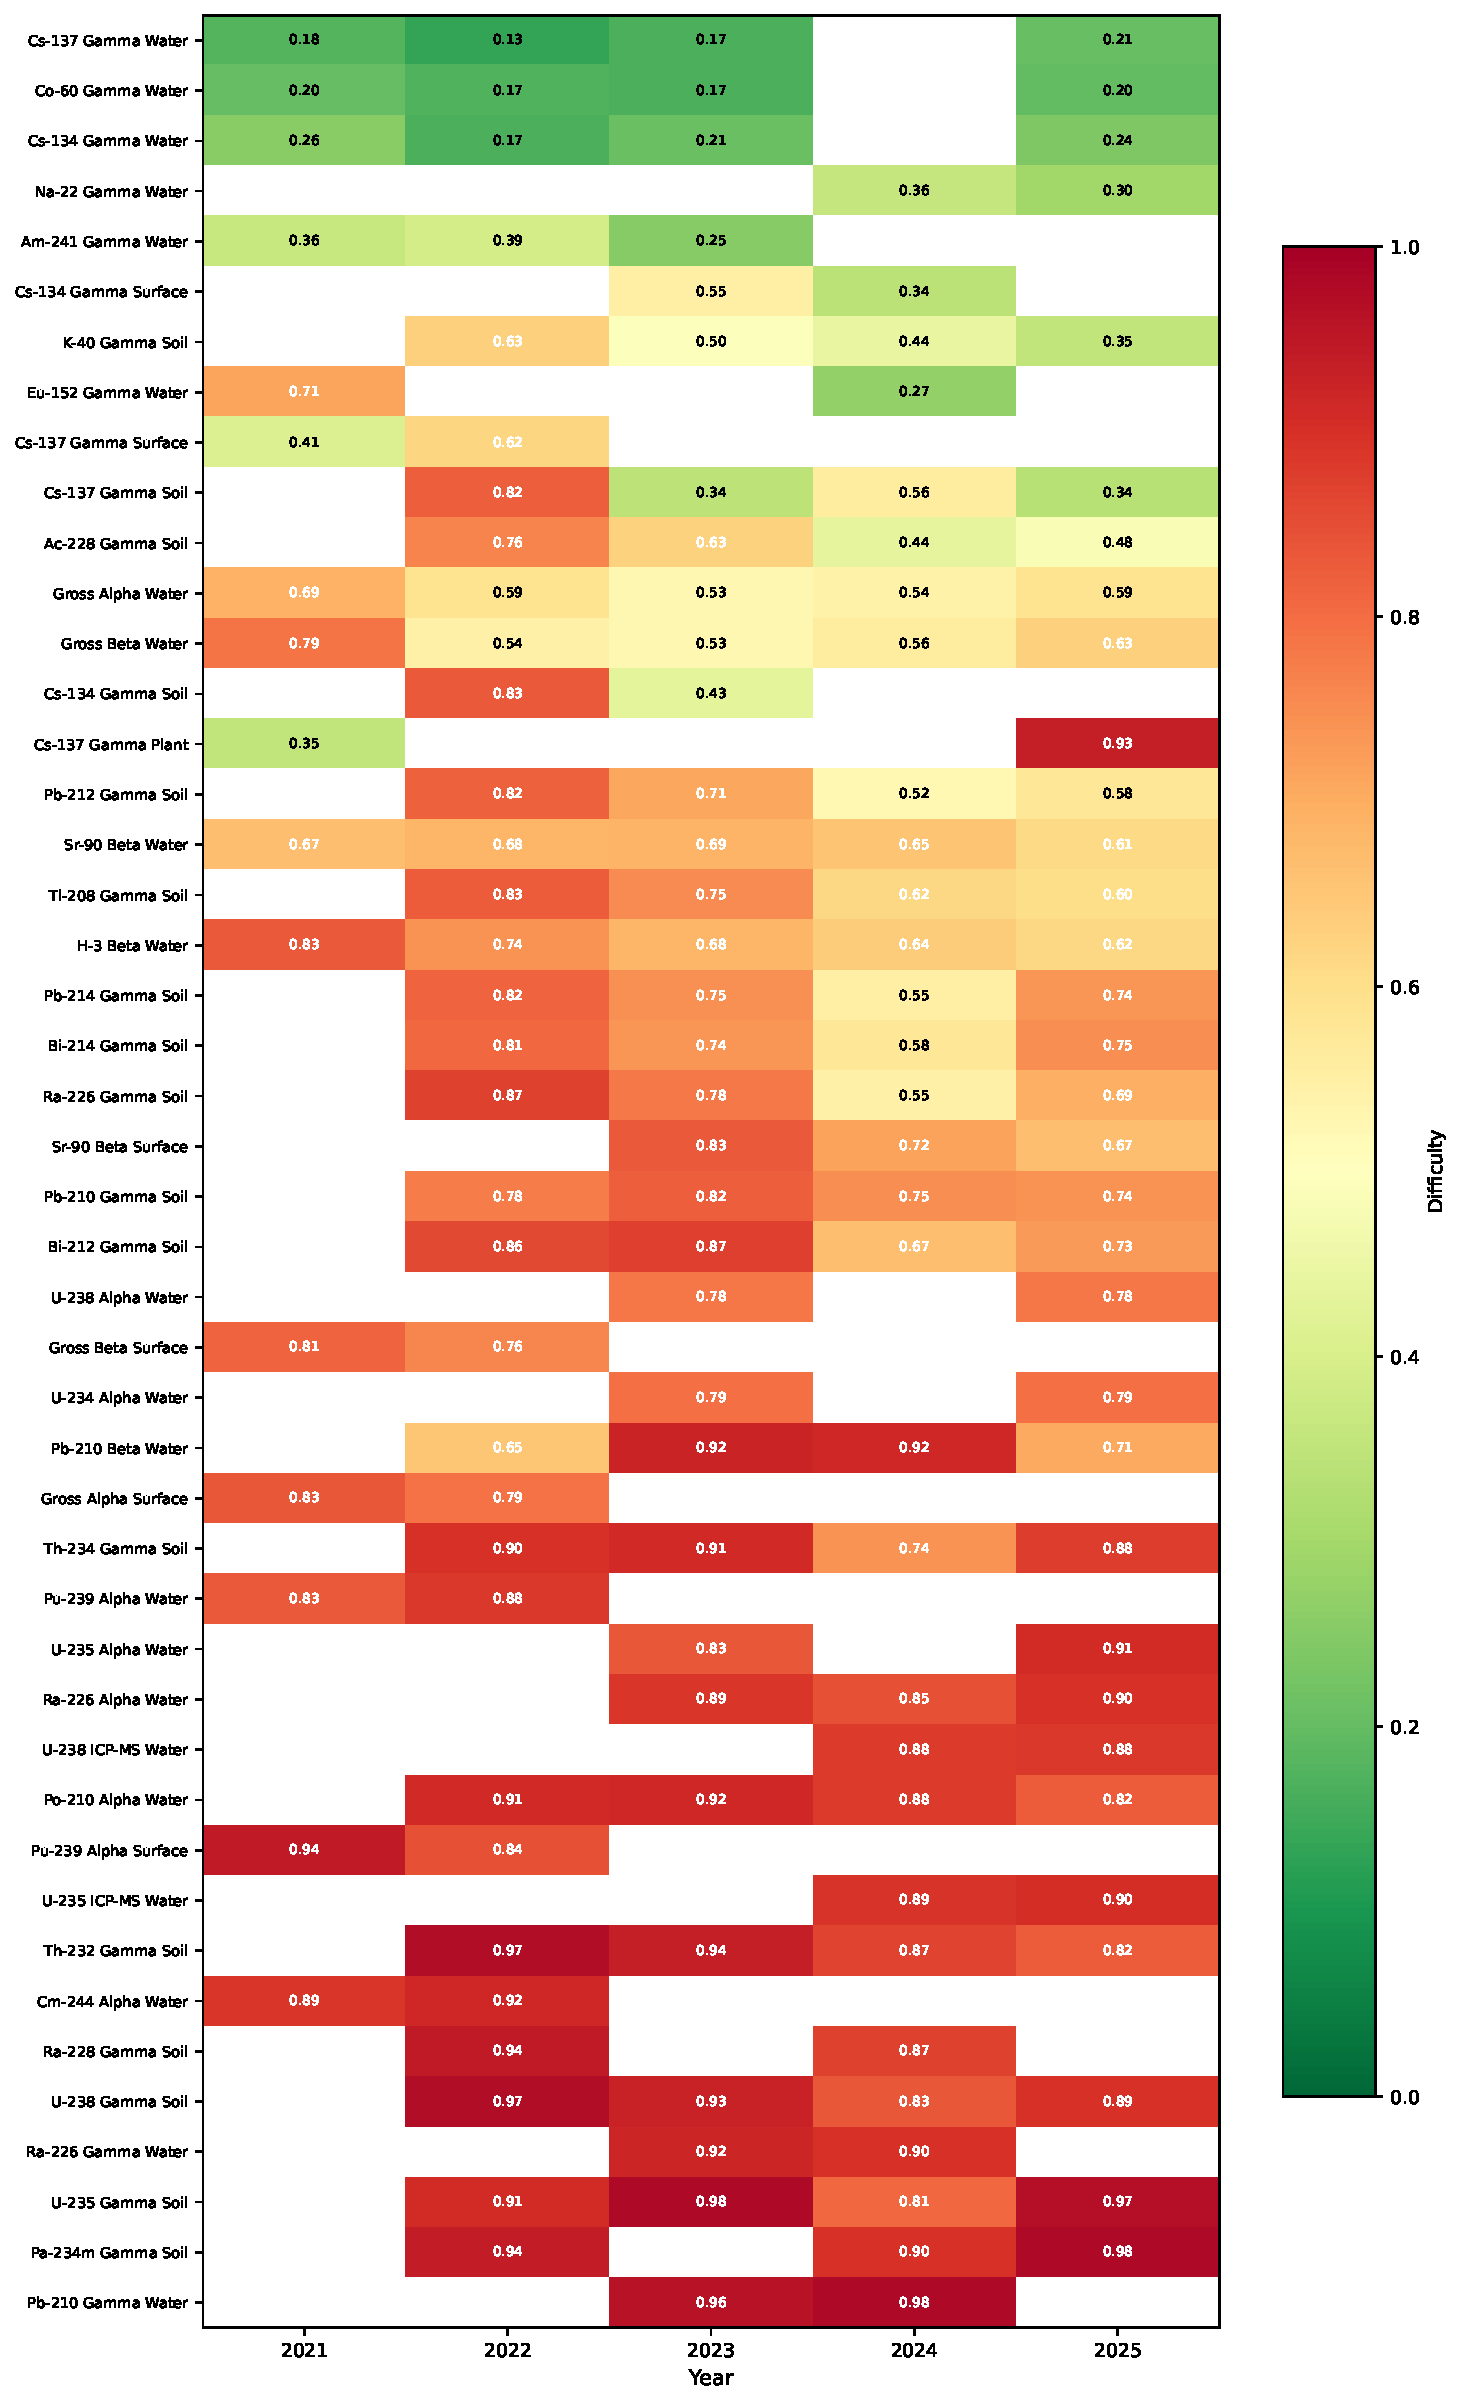
\includegraphics[width=0.98\textwidth]{figures/fig_difficulty_heatmap.pdf}
  \caption{Heatmap of project difficulty coefficients by nuclide--matrix combination (rows) and year (columns). Cells are color-coded from green ($D = 0$, 100\% pass) to red ($D = 1$, 0\% pass). White cells indicate years in which the project was not offered or fewer than two laboratories participated.}
  \label{fig:difficulty_heatmap}
\end{figure}

\subsection{Laboratory Performance Comparison}
\label{sec:lab_performance}

Figure~\ref{fig:lab_performance} summarizes the case-study laboratory's participation breadth relative to the global pool. The number of projects in which the laboratory participated increased from 12 (2021) to 35 (2025), representing a nearly threefold expansion in analytical scope. This expansion reflects a deliberate strategy of progressively adding new radionuclide--matrix capabilities to the laboratory's accredited scope. When ranked by participation breadth, the laboratory improved from \#187/270 in 2021 to \#4/399 in 2025. The ranking by the number of ``A'' (Acceptable) scores achieved (which, given the near-perfect pass rate, is essentially a participation-breadth metric rather than an independent quality indicator) was correspondingly strong: \#2/399 in 2025. The more informative inter-laboratory comparisons are the within-project percentile rankings (Figure~\ref{fig:lab_percentile_ranking}) and the RDI-based rankings (Section~\ref{sec:rdi}), which normalize for the number of projects and reflect analytical accuracy rather than scope breadth.

\begin{figure}[H]
  \centering
  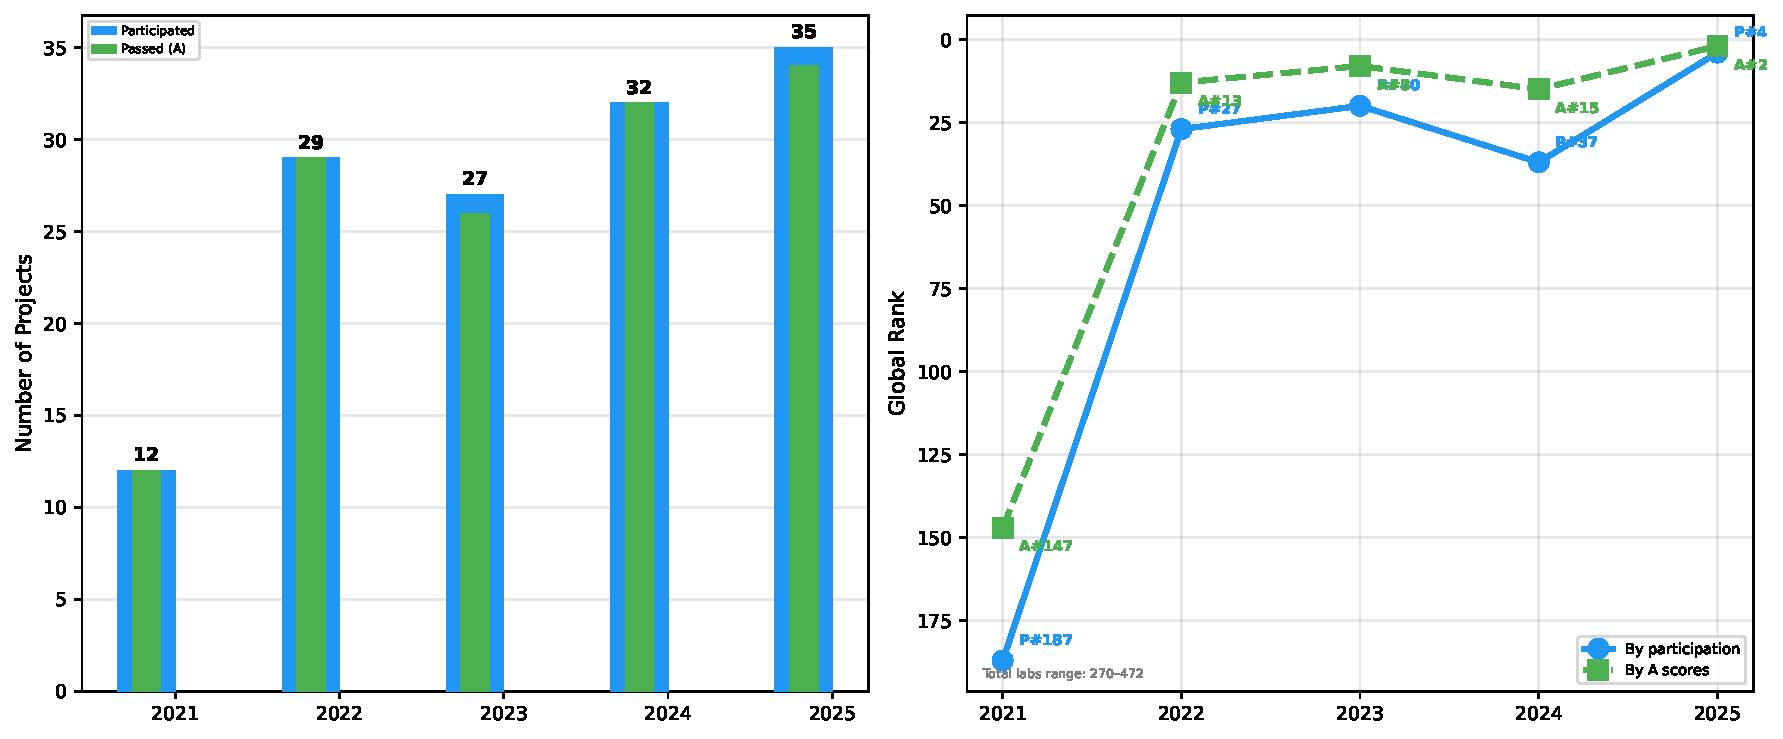
\includegraphics[width=0.98\textwidth]{figures/fig_lab_performance.pdf}
  \caption{(a) Number of projects participated versus passed by our laboratory in each year. (b) Global ranking of our laboratory by participation breadth (blue) and by number of Acceptable scores (green). Tied ranks (``min'' method) are used. The A-count rank is consistently stronger: \#2 globally in 2025.}
  \label{fig:lab_performance}
\end{figure}

The pass rate was 100\% in 2021 (12/12), 2022 (29/29), and 2024 (32/32), and 96.3\% in 2023 (26/27) and 97.1\% in 2025 (34/35). The two ``Warning'' scores---Sr-90 Beta Surface in 2023~\cite{kavasi2019} and U-235 Gamma Water in 2025---each corresponded to $|Z\text{-score}|$ values between 2 and 3, marginally outside the ``Acceptable'' range. No ``Not Acceptable'' (N) score was recorded across all 135 measurements.

Figure~\ref{fig:lab_percentile_ranking} presents the distribution of our laboratory's within-project percentile ranks, aggregated by year as box-and-whisker plots. The overall mean percentile rank across all 109 project participations with reported relative bias was 23.8\% (95\% bootstrap CI: 20.4\%--27.2\%), indicating that for the average project, our absolute relative bias was lower than approximately 76\% of peer laboratories. A Wilcoxon signed-rank test confirmed that our laboratory's absolute relative bias was significantly lower than the all-laboratory median across projects ($W = 389$, $p < 0.001$, $n = 109$; 97 of 109 below median). The year-to-year variation in median percentile rank (ranging from 12.6\% in 2022 to 32.5\% in 2025) was not statistically significant (Kruskal--Wallis $H = 7.29$, $p = 0.12$), and a Mann--Kendall test on annual means detected no significant trend ($p = 0.81$). These results indicate a consistent pattern of above-median accuracy rather than a directional change over time.

\begin{figure}[H]
  \centering
  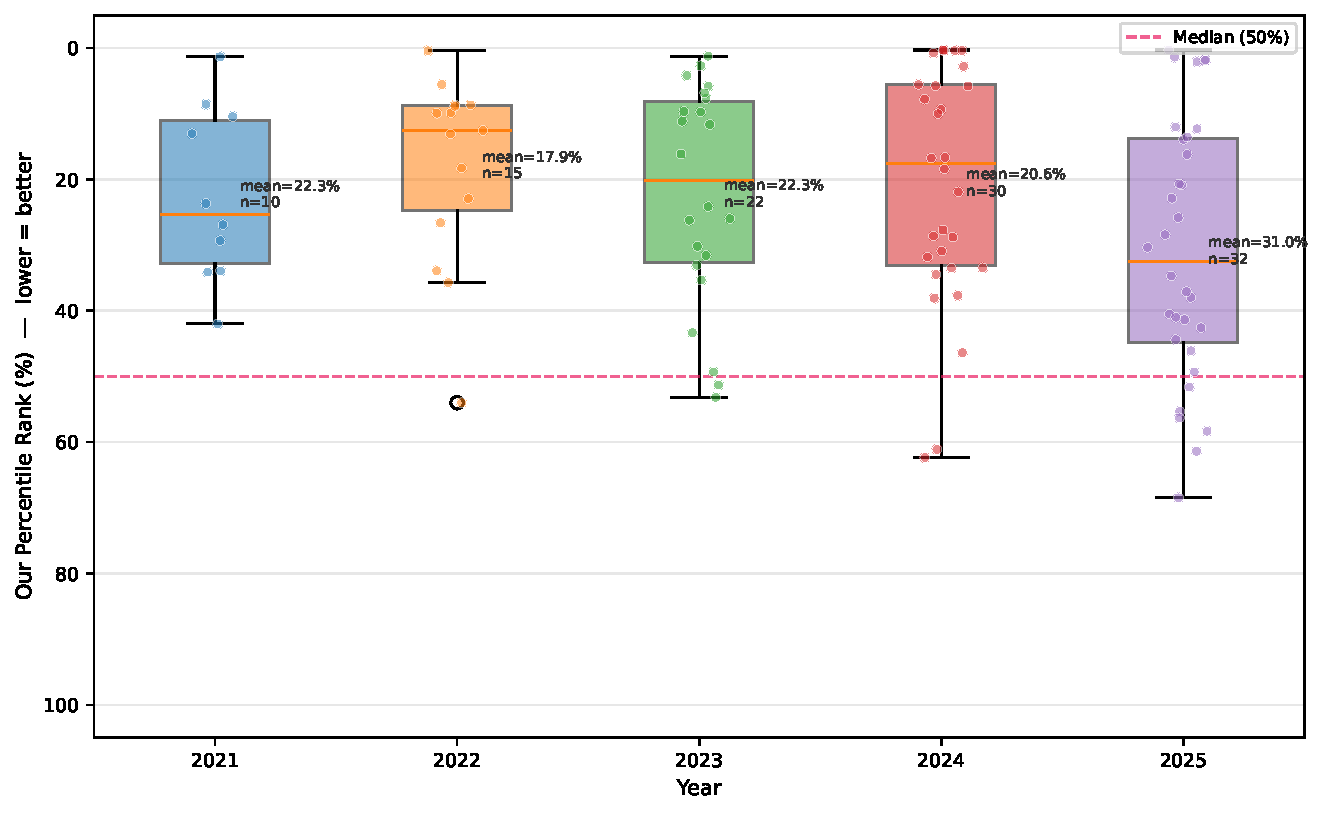
\includegraphics[width=0.95\textwidth]{figures/fig_lab_percentile_ranking.pdf}
  \caption{Yearly distribution of our laboratory's within-project percentile ranks (2021--2025). Each boxplot summarizes one year: box = IQR, center line = median, whiskers = 1.5$\times$IQR. Jittered points represent individual projects. The red dashed line at 50\% marks the global median reference. Lower values indicate fewer laboratories outperformed ours (better accuracy). Annotations show the annual mean and number of projects.}
  \label{fig:lab_percentile_ranking}
\end{figure}

\subsection{Performance Across Difficulty Tiers}
\label{sec:difficulty_tiers}

A crucial question for any PT participant is whether its strong pass rate holds only for easy projects or extends across the full difficulty spectrum. Figure~\ref{fig:tier_counts} stratifies our laboratory's projects by difficulty tier for each year, and also shows—as a gray reference bar—the total number of distinct IAEA projects offered in that tier that year, providing context for our laboratory's coverage breadth.

\begin{figure}[H]
  \centering
  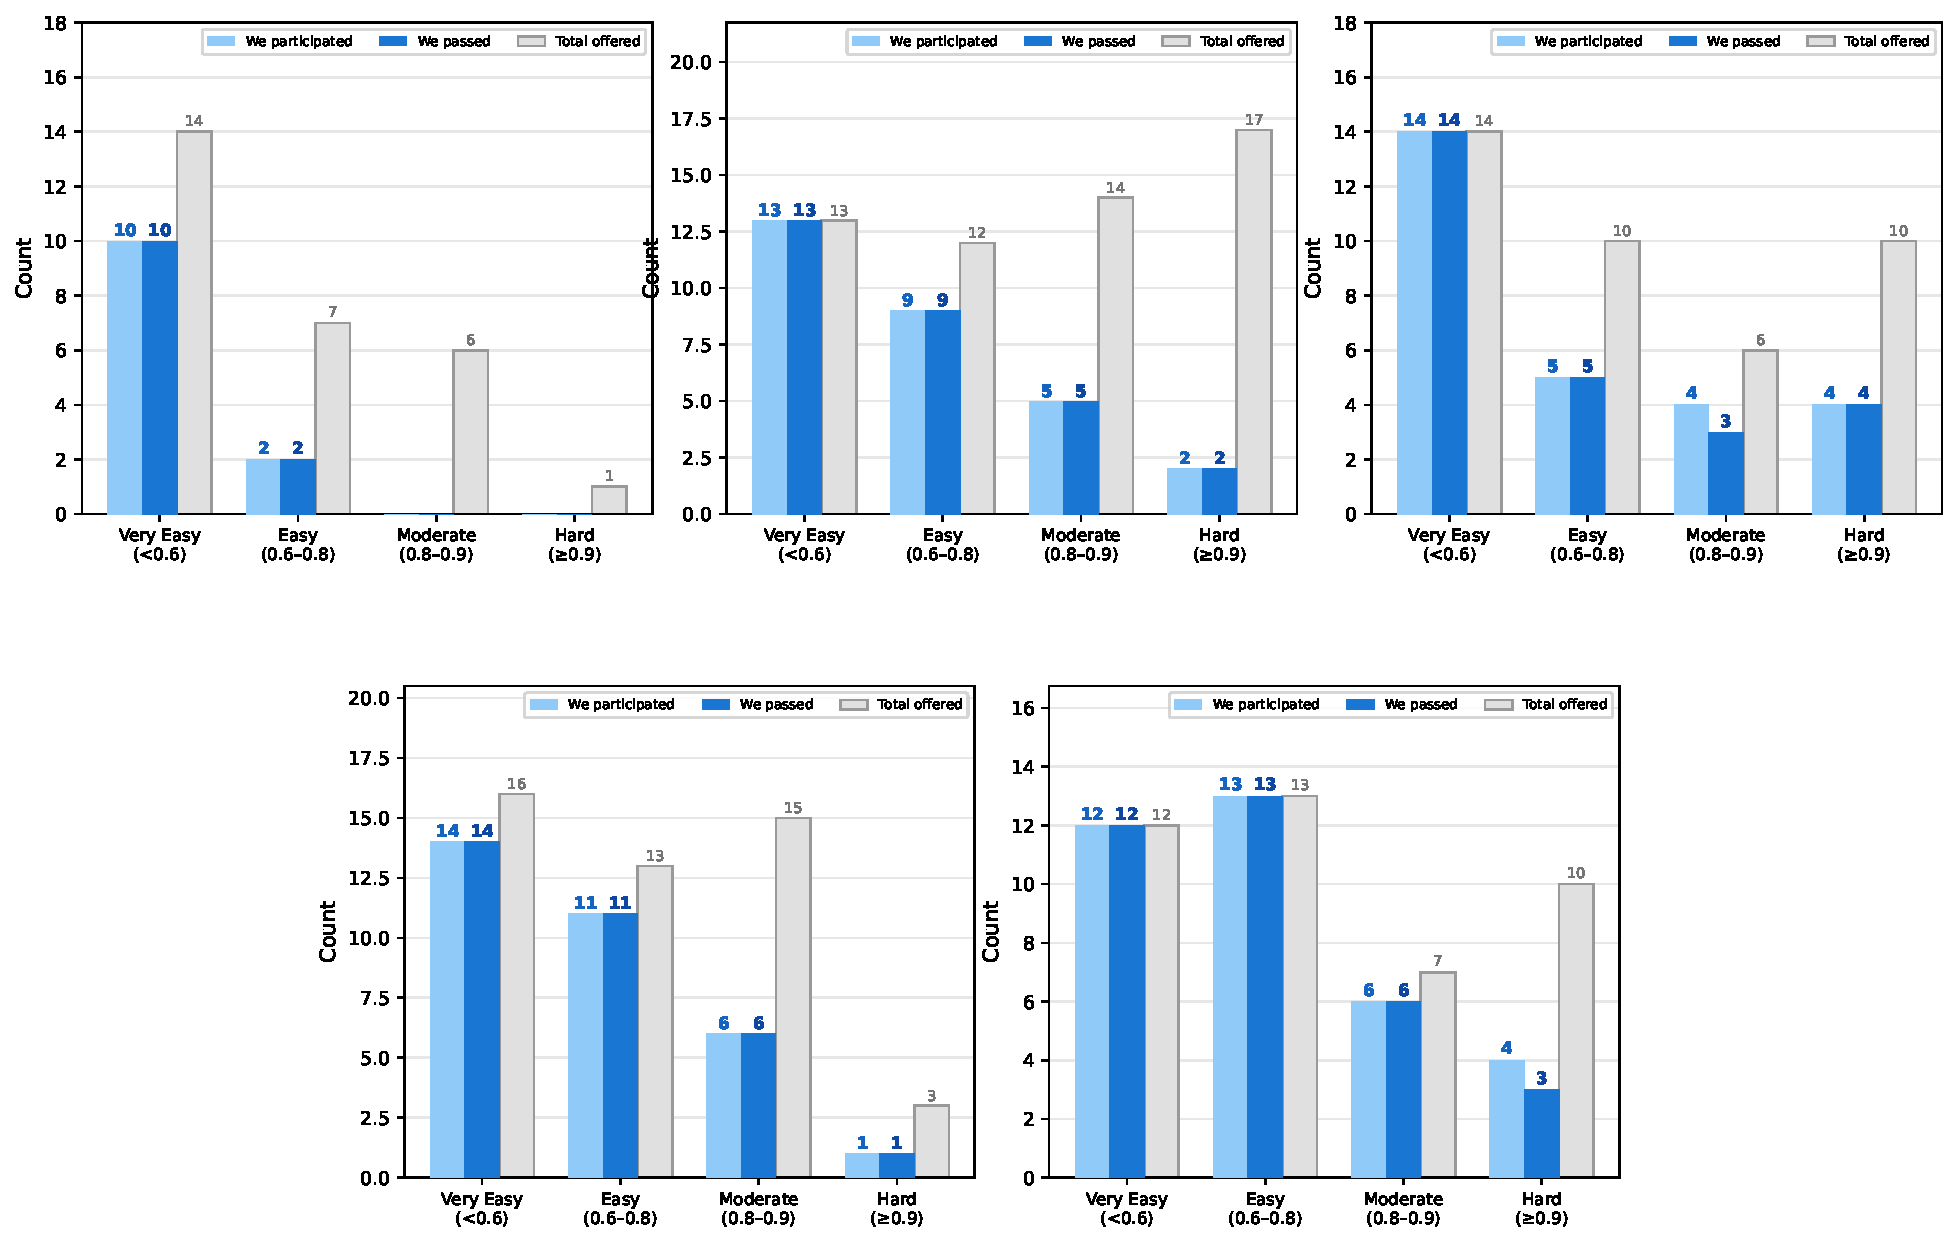
\includegraphics[width=0.98\textwidth]{figures/fig_difficulty_tier_counts.pdf}
  \caption{Number of projects by difficulty tier for each year. Light blue bars: our laboratory's participated projects; dark blue bars: projects passed (scored ``A''); gray bars: total distinct IAEA projects in that tier (whether we participated or not). The ``our $n$'' in each subplot title indicates the total number of projects our laboratory participated in that year.}
  \label{fig:tier_counts}
\end{figure}

The results demonstrate robust performance across the difficulty spectrum. In the Very Easy ($D < 0.6$) and Easy ($0.6 \leq D \leq 0.8$) tiers, which collectively account for 85.9\% of our total participations, the pass rate was 100\% across all five years. In the Moderate tier ($0.8 < D \leq 0.9$, 10.4\% of participations), the pass rate was 95.0\% (19/20), with the single ``Warning'' occurring in 2023. In the Hard tier ($D > 0.9$, 8.9\% of participations), the pass rate was 91.7\% (11/12), with the single non-A score attributable to $^{235}$U. Importantly, our pass rate in the Hard tier substantially exceeded the global average for these challenging projects (Figure~\ref{fig:tier_pass_rate}).

\begin{figure}[H]
  \centering
  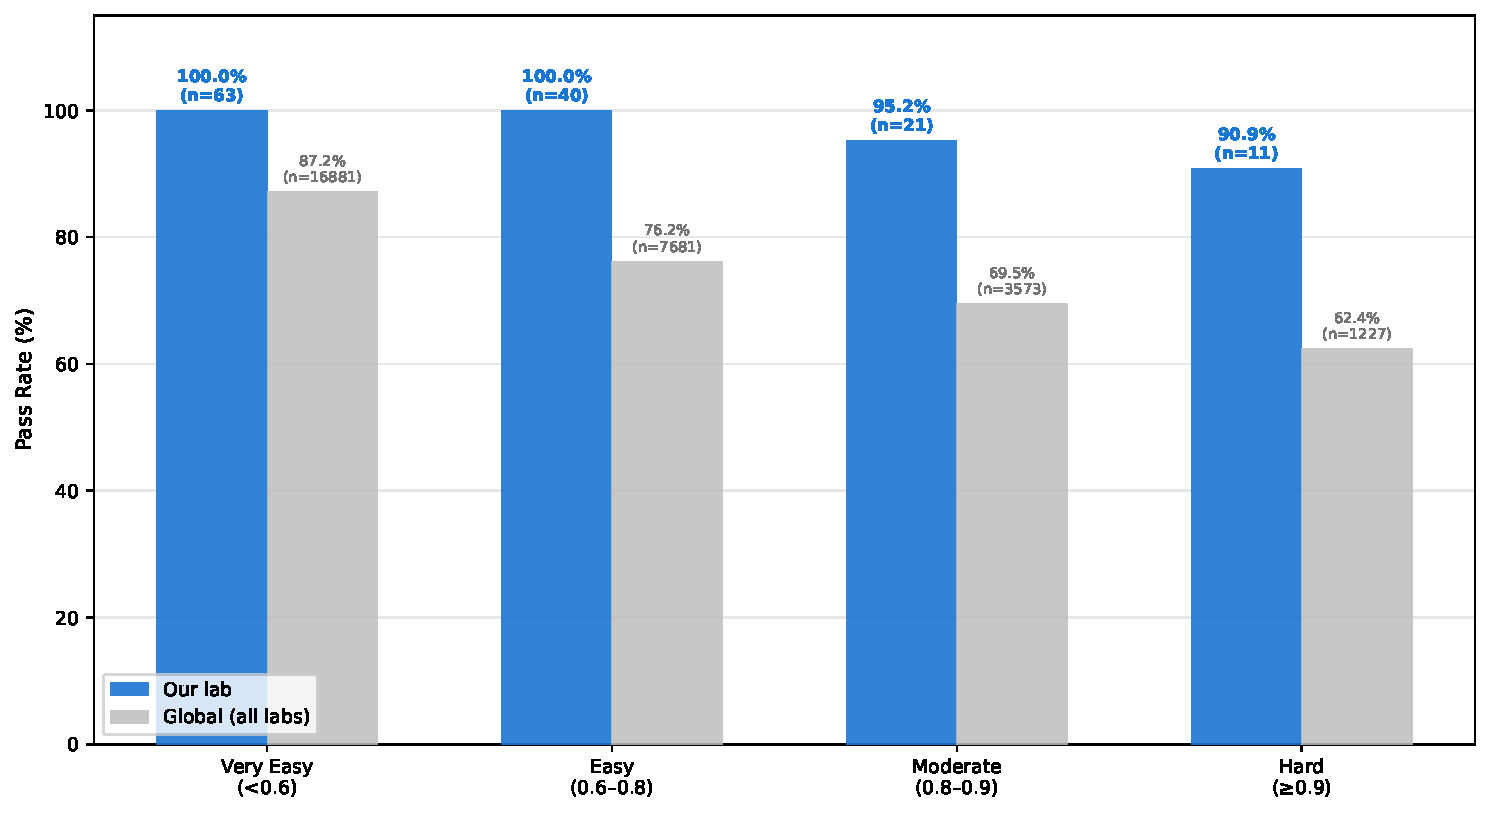
\includegraphics[width=0.90\textwidth]{figures/fig_difficulty_tier_pass_rate.pdf}
  \caption{Aggregated pass rate by difficulty tier (all years combined): our laboratory (blue) versus the global average across all participating laboratories (gray). The $n$ values indicate the number of project participations. Our laboratory consistently outperforms the global average, with the gap widest in the Hard tier.}
  \label{fig:tier_pass_rate}
\end{figure}

\subsection{Result Deviation Index (RDI) Analysis}
\label{sec:rdi}

Table~\ref{tab:rdi_summary} presents our laboratory's weighted RDI. The MARB-based weighting reduces the influence of inherently high-uncertainty projects. Our weighted RDI ranged from 1.41\% (2021) to 4.66\% (2025), with the 5-year mean at 3.05\%. The apparent increase from 2021 to 2025 was not statistically significant by the Mann--Kendall test ($S = 8$, $p = 0.086$), though the borderline $p$-value and the monotonic increase in four of five years suggest this should be monitored as additional years of data become available. The increased RDI in later years coincides with the threefold expansion in the number of participated projects with reported bias (from 10 in 2021 to 32 in 2025). A Spearman correlation analysis between RDI and participation breadth across all laboratories showed a weak and inconsistent relationship ($\rho$ ranged from $-0.12$ to $+0.14$ across years), suggesting that RDI is not systematically inflated by participating in more projects.

\begin{table}[H]
\centering
\caption{Result Deviation Index (RDI) of the case-study laboratory compared with all-laboratory benchmarks.}
\label{tab:rdi_summary}
\resizebox{\linewidth}{!}{
\begin{tabular}{@{}lccccccc@{}}
\toprule
\textbf{Year} & \textbf{$n$\textsuperscript{a}} & \textbf{RDI\textsubscript{w}} & \textbf{RDI\textsubscript{uw}} & \textbf{SEM} & \textbf{Median $|$bias$|$} & \textbf{Rank} & \textbf{Labs\textsuperscript{b}} \\
 &  & \textbf{(\%)} & \textbf{(\%)} & \textbf{(\%)} & \textbf{(\%)} & & \\
\midrule
2021 & 10 & 1.41 & 1.46 & 0.28 & 1.34 & \#4  & 259 \\
2022 & 15 & 2.03 & 2.16 & 0.51 & 1.44 & \#15 & 265 \\
2023 & 22 & 3.97 & 4.13 & 1.26 & 2.08 & \#34 & 315 \\
2024 & 30 & 3.16 & 3.42 & 0.71 & 1.45 & \#15 & 468 \\
2025 & 32 & 4.66 & 4.82 & 0.67 & 4.95 & \#52 & 392 \\
\midrule
5-yr mean & -- & 3.05 & 3.20 & -- & 2.30 & -- & -- \\
\bottomrule
\end{tabular}
}
\par\vspace{4pt}\footnotesize
\textsuperscript{a}Projects with reported relative bias (total participations: 12, 29, 27, 32, 35 in 2021--2025).
\textsuperscript{b}Labs with $\geq 1$ reported rel.\ bias value. Excluded labs (projects without rel.\ bias only): 11, 12, 4, 4, 7 (2021--2025).\\
RDI\textsubscript{w} = weighted ($w_k = 1.2/(1+\text{MARB}_k/100\%)$); RDI\textsubscript{uw} = unweighted ($w_k = 1.0$). SEM = standard error of RDI\textsubscript{w}.
\end{table}

To evaluate the sensitivity of the RDI to the choice of weighting function, we compared three alternatives: the proposed weighted RDI ($w_k = 1.2/(1+\text{MARB}_k/100\%)$), an unweighted RDI ($w_k \equiv 1.0$), and an inverse-MARB scheme ($w_k = 20\%/\text{MARB}_k$, clipped to $[0.5, 2.0]$). The 5-year mean RDI was 3.05\% (weighted), 3.20\% (unweighted), and 2.55\% (inverse-MARB). The weighted and unweighted rankings were nearly identical: the laboratory's RDI rank shifted by at most 2 positions across all five years (Table~\ref{tab:rdi_summary}). The inverse-MARB scheme produced lower RDI values because it applies stronger down-weighting to high-MARB projects, but the rank ordering was similarly stable. These results indicate that the RDI framework's conclusions are robust to the choice of weighting function; the key finding---that the laboratory's RDI is consistently below the all-laboratory mean---holds under all three schemes.

It is important to note that 26 of the 135 measurements (19\%) had no reported relative bias and were therefore excluded from RDI computations (Table~\ref{tab:rdi_summary}, footnote \textsuperscript{a}). The excluded projects were predominantly gross alpha/beta measurements and a subset of gamma-emitting nuclides in soil matrices. In 2022, only 29\% of the 57 PT projects had MARB values available; for the remaining 71\%, a default weight of $w = 1.0$ (equivalent to $\text{MARB} = 20\%$) was used. The missing-MARB rate was lower in other years (0\%--25\%). The laboratories excluded from the RDI ranking pool (1\%--4\% of participants per year, Table~\ref{tab:rdi_summary} footnote \textsuperscript{b}) were those that exclusively participated in projects without reported relative bias; their exclusion introduces a small but unquantified selection effect.

Figure~\ref{fig:rdi_trend} plots the laboratory's RDI against the all-laboratory benchmark band. For all five years, the RDI fell below the all-laboratory mean, confirming consistently better-than-average accuracy under all weighting schemes examined. The scatter plots (e.g., Figure~\ref{fig:rdi_scatter}) have y-axes capped at 100\% for readability; benchmark reference lines are computed from the visible subset (laboratories with $\text{RDI} \leq 100\%$).

\begin{figure}[H]
  \centering
  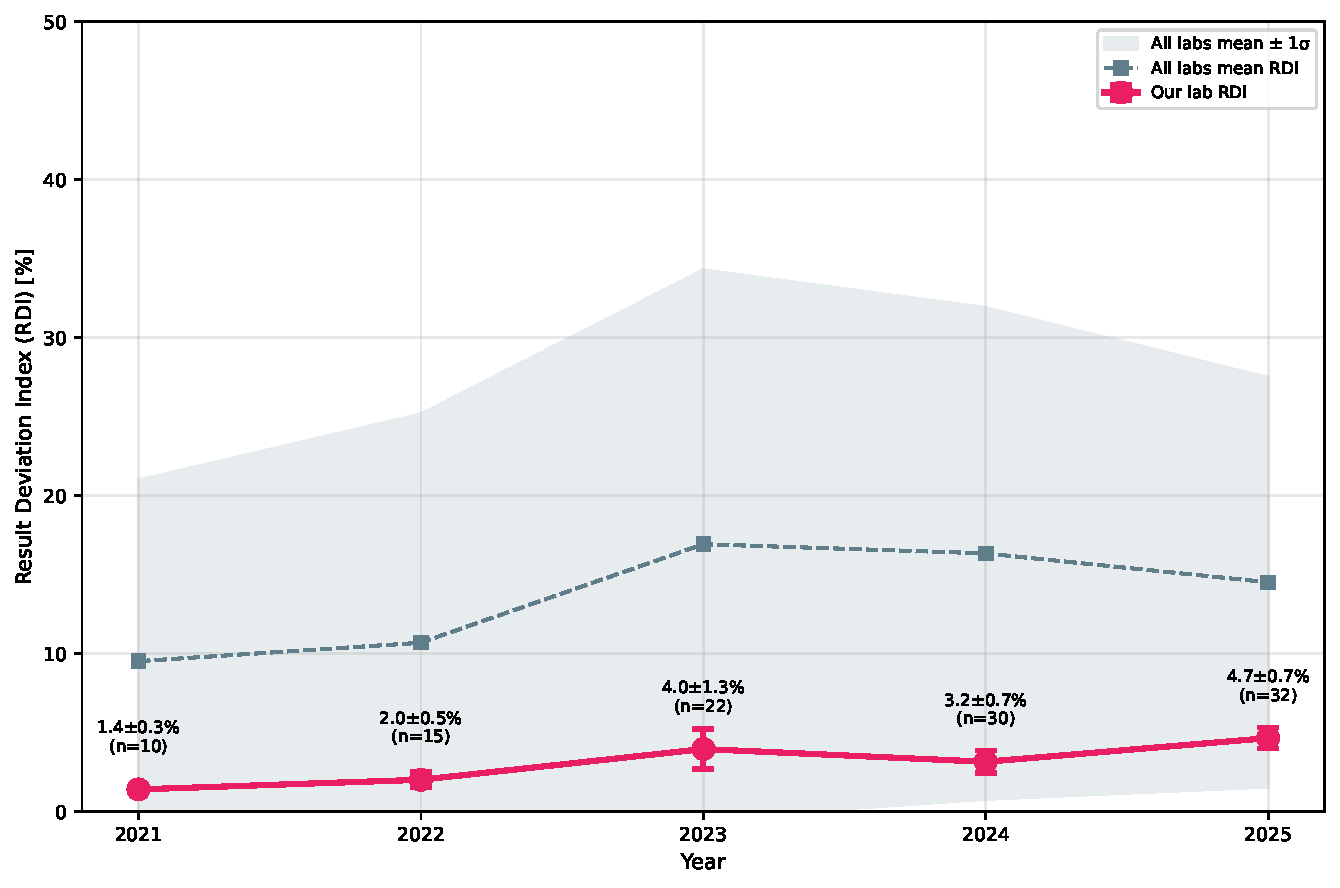
\includegraphics[width=0.95\textwidth]{figures/fig_rdi_trend.pdf}
  \caption{Trend of our laboratory's Result Deviation Index (RDI) compared with the all-laboratory mean RDI (dashed line) and $\pm 1\sigma$ band (shaded region). Despite an increasing RDI in recent years, our laboratory has remained consistently below the global benchmark.}
  \label{fig:rdi_trend}
\end{figure}

Figure~\ref{fig:rdi_scatter} shows a representative scatter plot of per-laboratory RDI values for 2025. Individual laboratories are sorted by RDI along the x-axis; the size of each point encodes the number of projects participated in. Our laboratory is prominently visible in the lower region.

\begin{figure}[H]
  \centering
  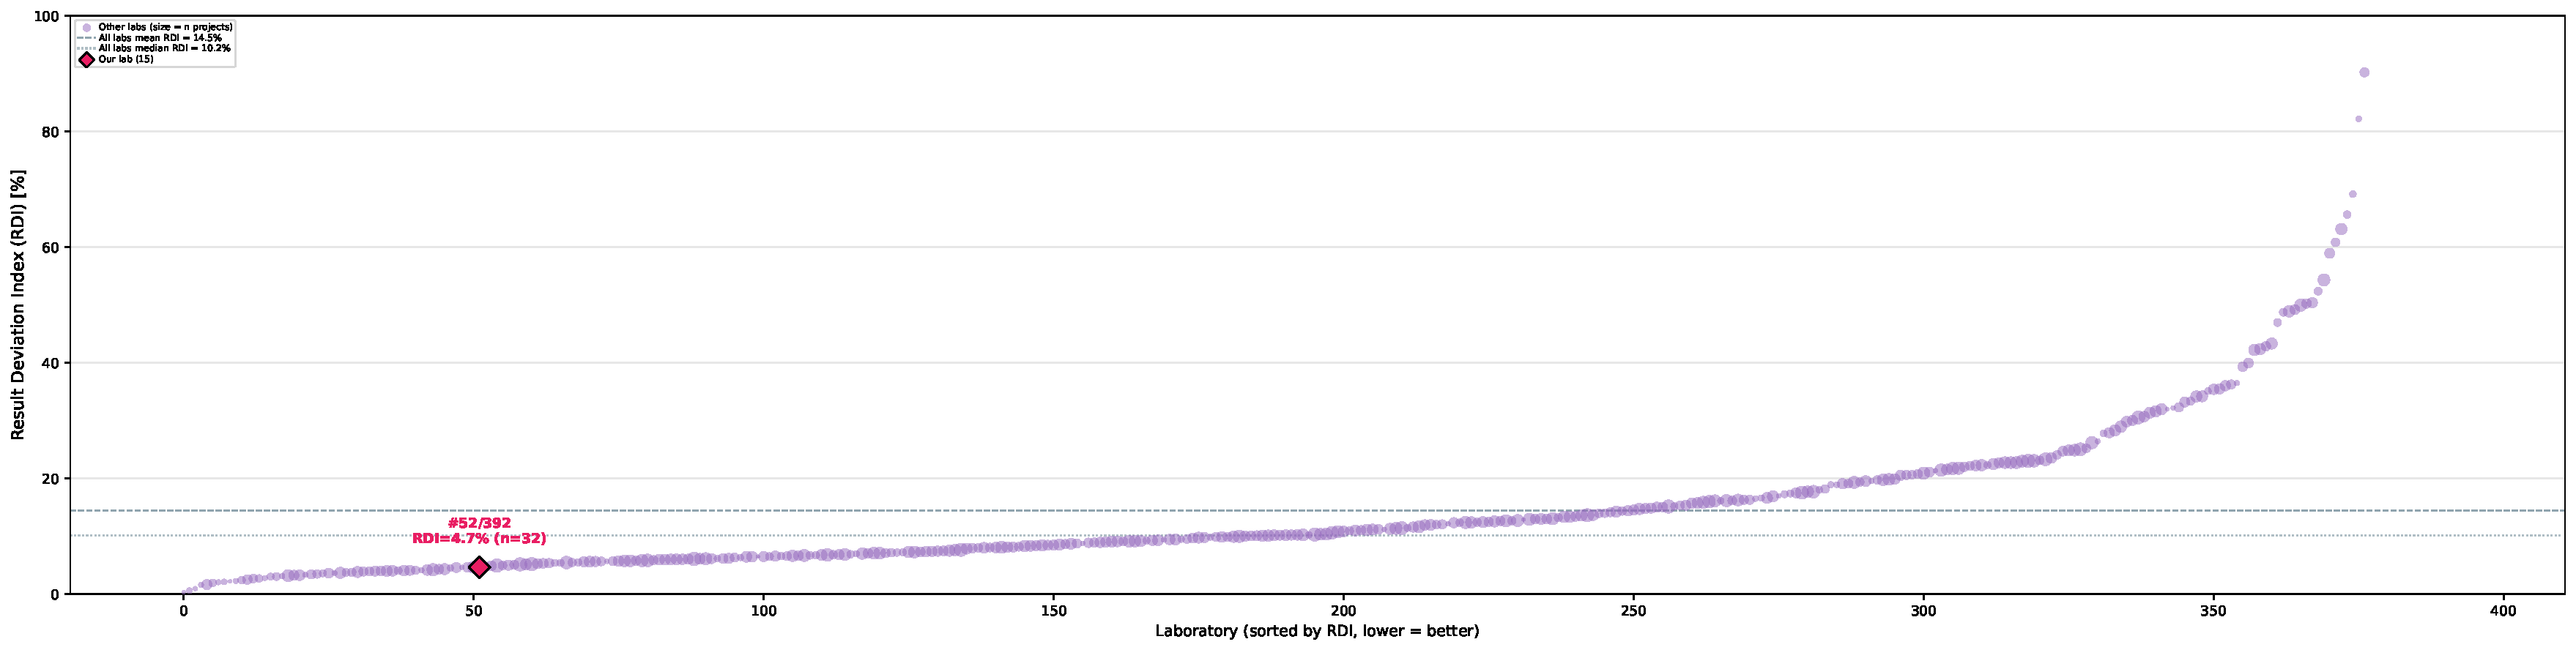
\includegraphics[width=0.95\textwidth]{figures/fig_rdi_scatter_2025.pdf}
  \caption{Result Deviation Index by laboratory for the 2025 round. Each point represents one laboratory; point size encodes number of projects. Pink diamond = our laboratory. Dashed and dotted lines show the all-laboratory mean and median RDI (computed from laboratories with RDI $\leq 100\%$). The y-axis is capped at 100\% for readability.}
  \label{fig:rdi_scatter}
\end{figure}

The RDI ranking plot (Figure~\ref{fig:rdi_ranking}) shows our laboratory's position in the weighted-RDI-sorted list of all laboratories that reported relative bias values. The best ranking was in 2021 (\#4/259, top 1.5\%), followed by 2024 (\#15/468, top 3.2\%). Even the relatively weaker years---2023 and 2025---placed our laboratory in the top 13--15\% of all participants. While the rank appears to decline over time (from \#4 to \#52), this coincides with a more than threefold increase in the number of participated projects with reported bias (from 10 in 2021 to 32 in 2025). Since the RDI is an arithmetic mean, adding more projects mechanically increases the probability of including a project with larger absolute bias~\cite{pomme2022}. The weak Spearman correlations between RDI and participation breadth (see above) suggest that this dilution effect is modest, but the trend in RDI rank should be interpreted with caution.

\begin{figure}[H]
  \centering
  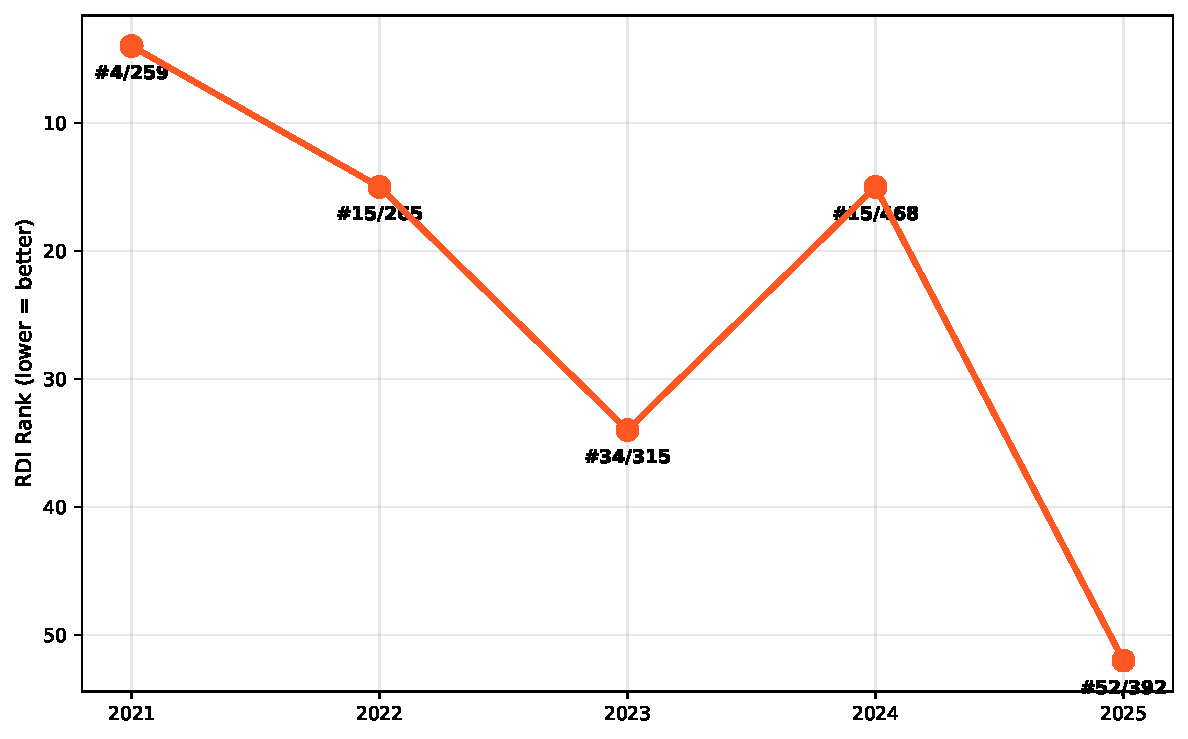
\includegraphics[width=0.85\textwidth]{figures/fig_rdi_ranking.pdf}
  \caption{Year-by-year weighted RDI ranking of our laboratory among all participating laboratories with reported relative bias values. The marked improvement from 2023 to 2024 coincides with the laboratory's expansion into sediment-matrix projects where competitive performance was achieved.}
  \label{fig:rdi_ranking}
\end{figure}

The RDI boxplot for our laboratory (Figure~\ref{fig:rdi_boxplot}) reveals the within-year distribution of $|\text{relative bias}|$. The 2023 and 2025 rounds exhibit notably higher variance, driven by a handful of projects with $|\text{RB}|$ exceeding 10\%. These outliers correspond to $^{210}$Po (alpha spectrometry, water), $^{234}$U (alpha spectrometry, water), and certain uranium isotopes by gamma spectrometry—analytes known to present calibration challenges due to low-energy photons, complex peak deconvolution, or the need for tracer-based radiochemical separation~\cite{hou2008,currie1968}.

\begin{figure}[H]
  \centering
  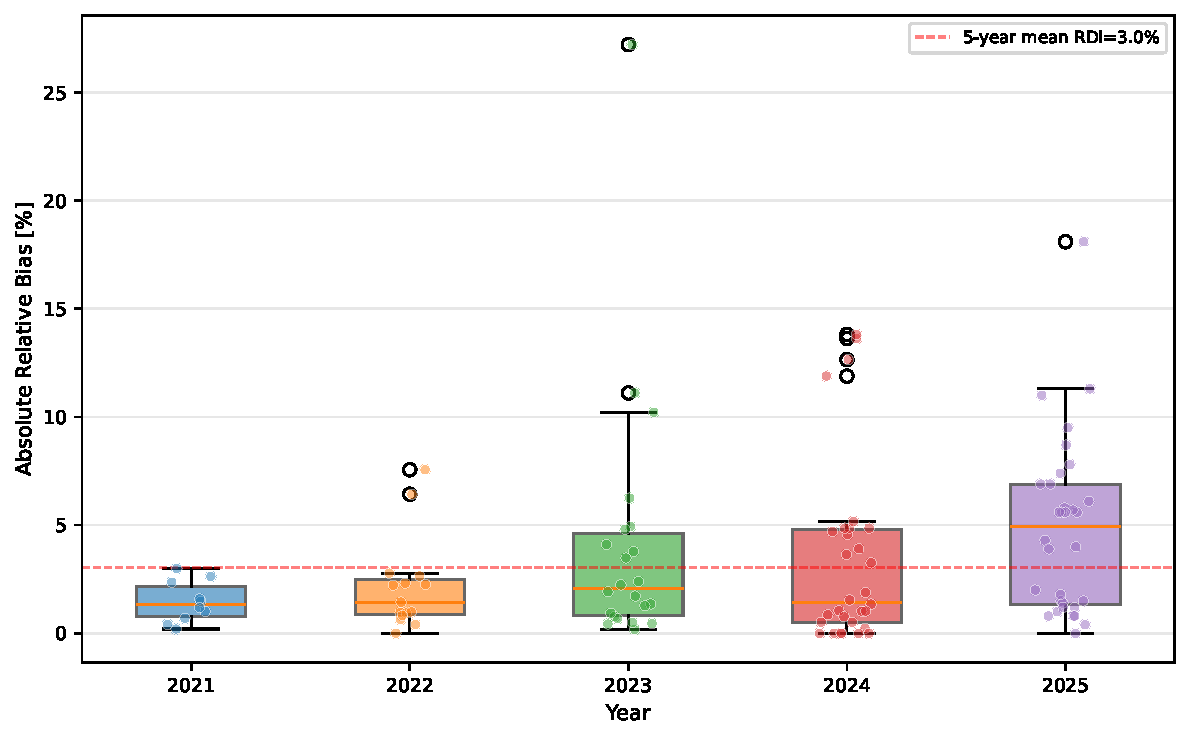
\includegraphics[width=0.90\textwidth]{figures/fig_rdi_boxplot.pdf}
  \caption{Boxplot of $|\text{relative bias}|$ for our laboratory across all projects within each year. The overlaid jittered points show individual project $|\text{RB}|$ values. The horizontal dashed line marks the 5-year weighted mean RDI (3.05\%).}
  \label{fig:rdi_boxplot}
\end{figure}

\subsection{Relative Bias Assessment and Within-Project Ranking}
\label{sec:relative_bias}

The heatmap in Figure~\ref{fig:relative_bias_heatmap} tracks our laboratory's relative bias for each nuclide--matrix combination across years. For the most frequently recurring projects—$^{137}$Cs in water, $^{134}$Cs in water, $^{60}$Co in water—the bias is consistently near zero (typically $|\text{RB}| < 2\%$), with no sign of directional drift over five years. This stability attests to the robustness of the laboratory's high-purity germanium (HPGe) gamma spectrometry calibration and quality control procedures~\cite{debertin1988}.

\begin{figure}[H]
  \centering
  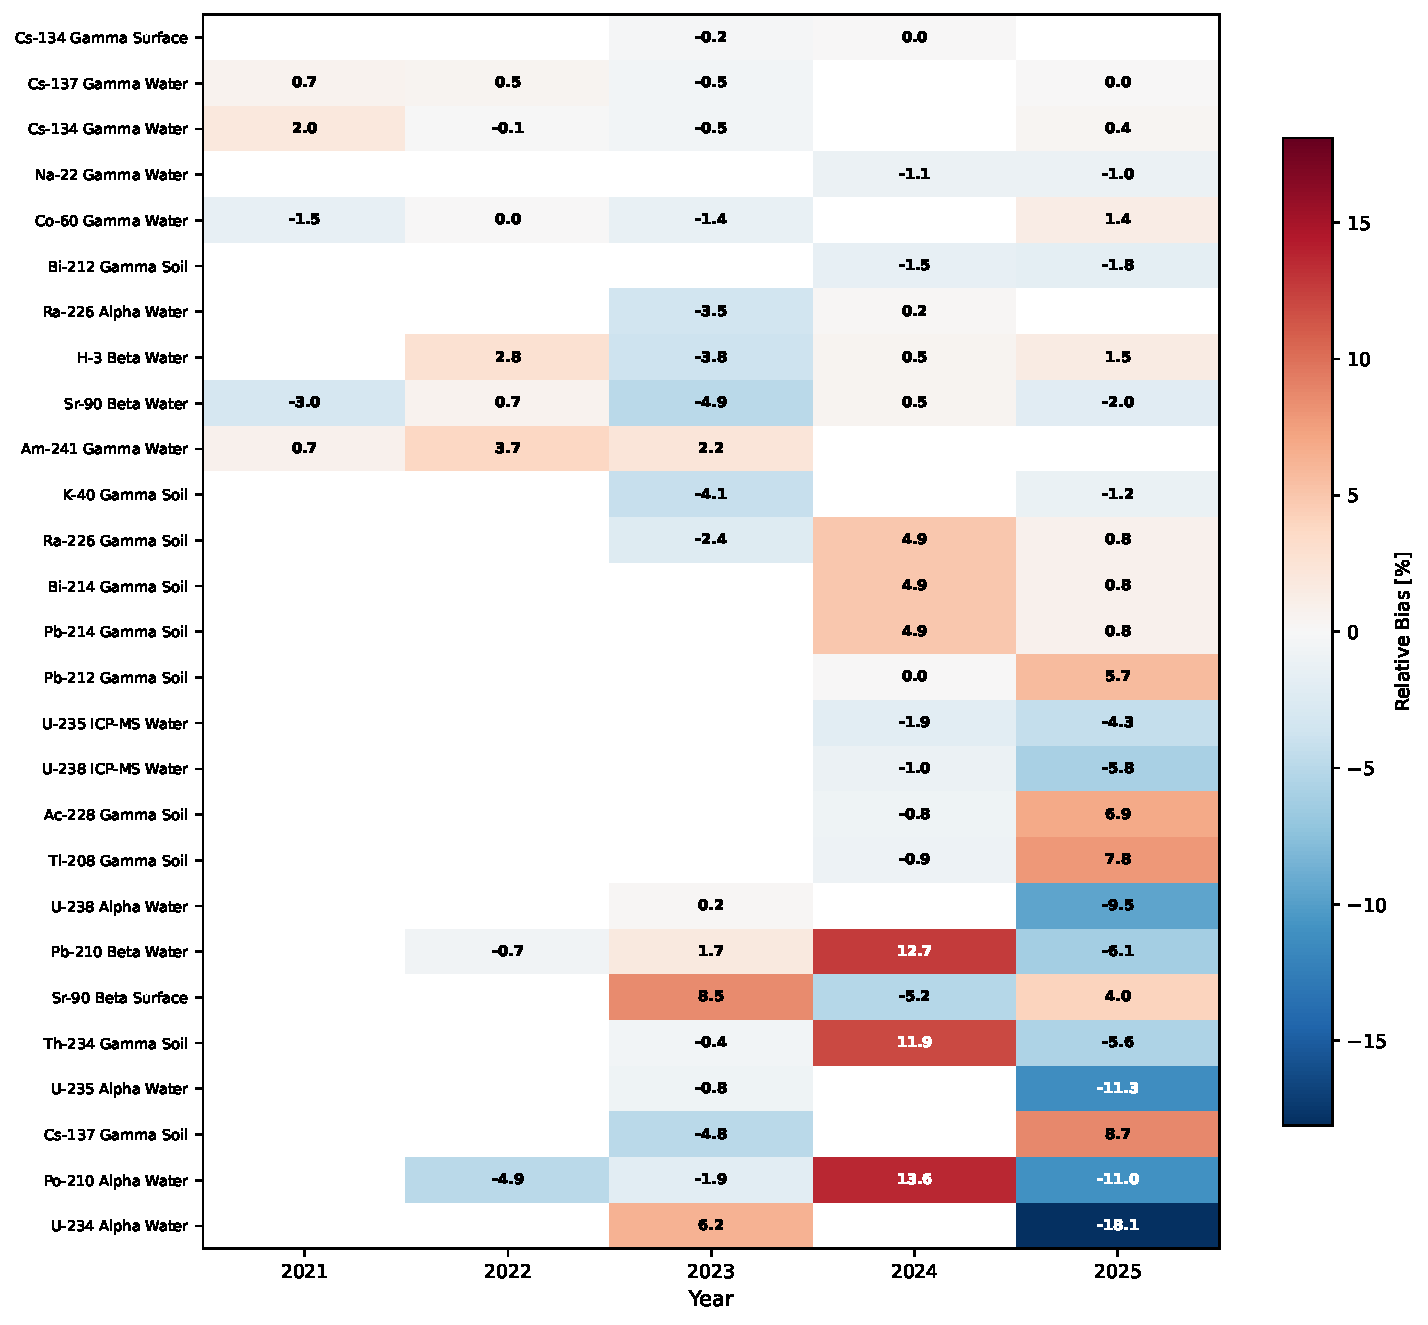
\includegraphics[width=0.98\textwidth]{figures/fig_relative_bias_heatmap.pdf}
  \caption{Relative bias heatmap for our laboratory across multi-year projects. The red--white--blue diverging color scale is centered at zero. Values near zero (white) indicate excellent agreement with the IAEA assigned value.}
  \label{fig:relative_bias_heatmap}
\end{figure}

Several projects exhibit consistently negative bias, warranting investigation of analyte-specific sources of systematic error. For $^{210}$Po (alpha spectrometry), negative bias may arise from incomplete auto-deposition yield onto silver discs, which is sensitive to pH, temperature, and the presence of interfering elements such as iron~\cite{matthews2007}. For $^{235}$U by gamma spectrometry, the low-energy 185.7 keV gamma line has a weak emission probability and can be interfered with by the $^{226}$Ra 186.2 keV line, requiring careful spectral deconvolution. For $^{235}$U and $^{238}$U by ICP-MS, accurate quantification depends on tracer equilibration and mass-bias correction. These technique-specific explanations suggest targeted corrective actions: deposition optimization for Po-210, interference verification for U-235 by gamma spectrometry, and tracer recovery audits for ICP-MS. The bias magnitudes for these nuclides ($-5\%$ to $-11\%$) are substantially smaller than the typical standard deviation for proficiency assessment (SDPA) values (often 15\%--20\%) used by the IAEA for Z-score calculation, which explains why these results still received ``A'' scores.

Figure~\ref{fig:relative_bias_2025_dist} shows the distribution of relative bias across all laboratories for each project our laboratory participated in during 2025, sorted by our laboratory's absolute deviation (smallest at top). Our laboratory (pink diamond) placed above the project median in 21 of 33 projects (63.6\%), with six in the top 5\%. The best performances were for $^{137}$Cs Gamma Water (rank \#1/339) and $^{134}$Cs Gamma Water (\#7/336). Across all five years, the mean percentile rank ranged from 17.9\% (2022) to 31.0\% (2025). The weakest performances involved $^{234}$U by alpha spectrometry and $^{137}$Cs in soil, though these still received ``A'' scores.

\begin{figure}[H]
  \centering
  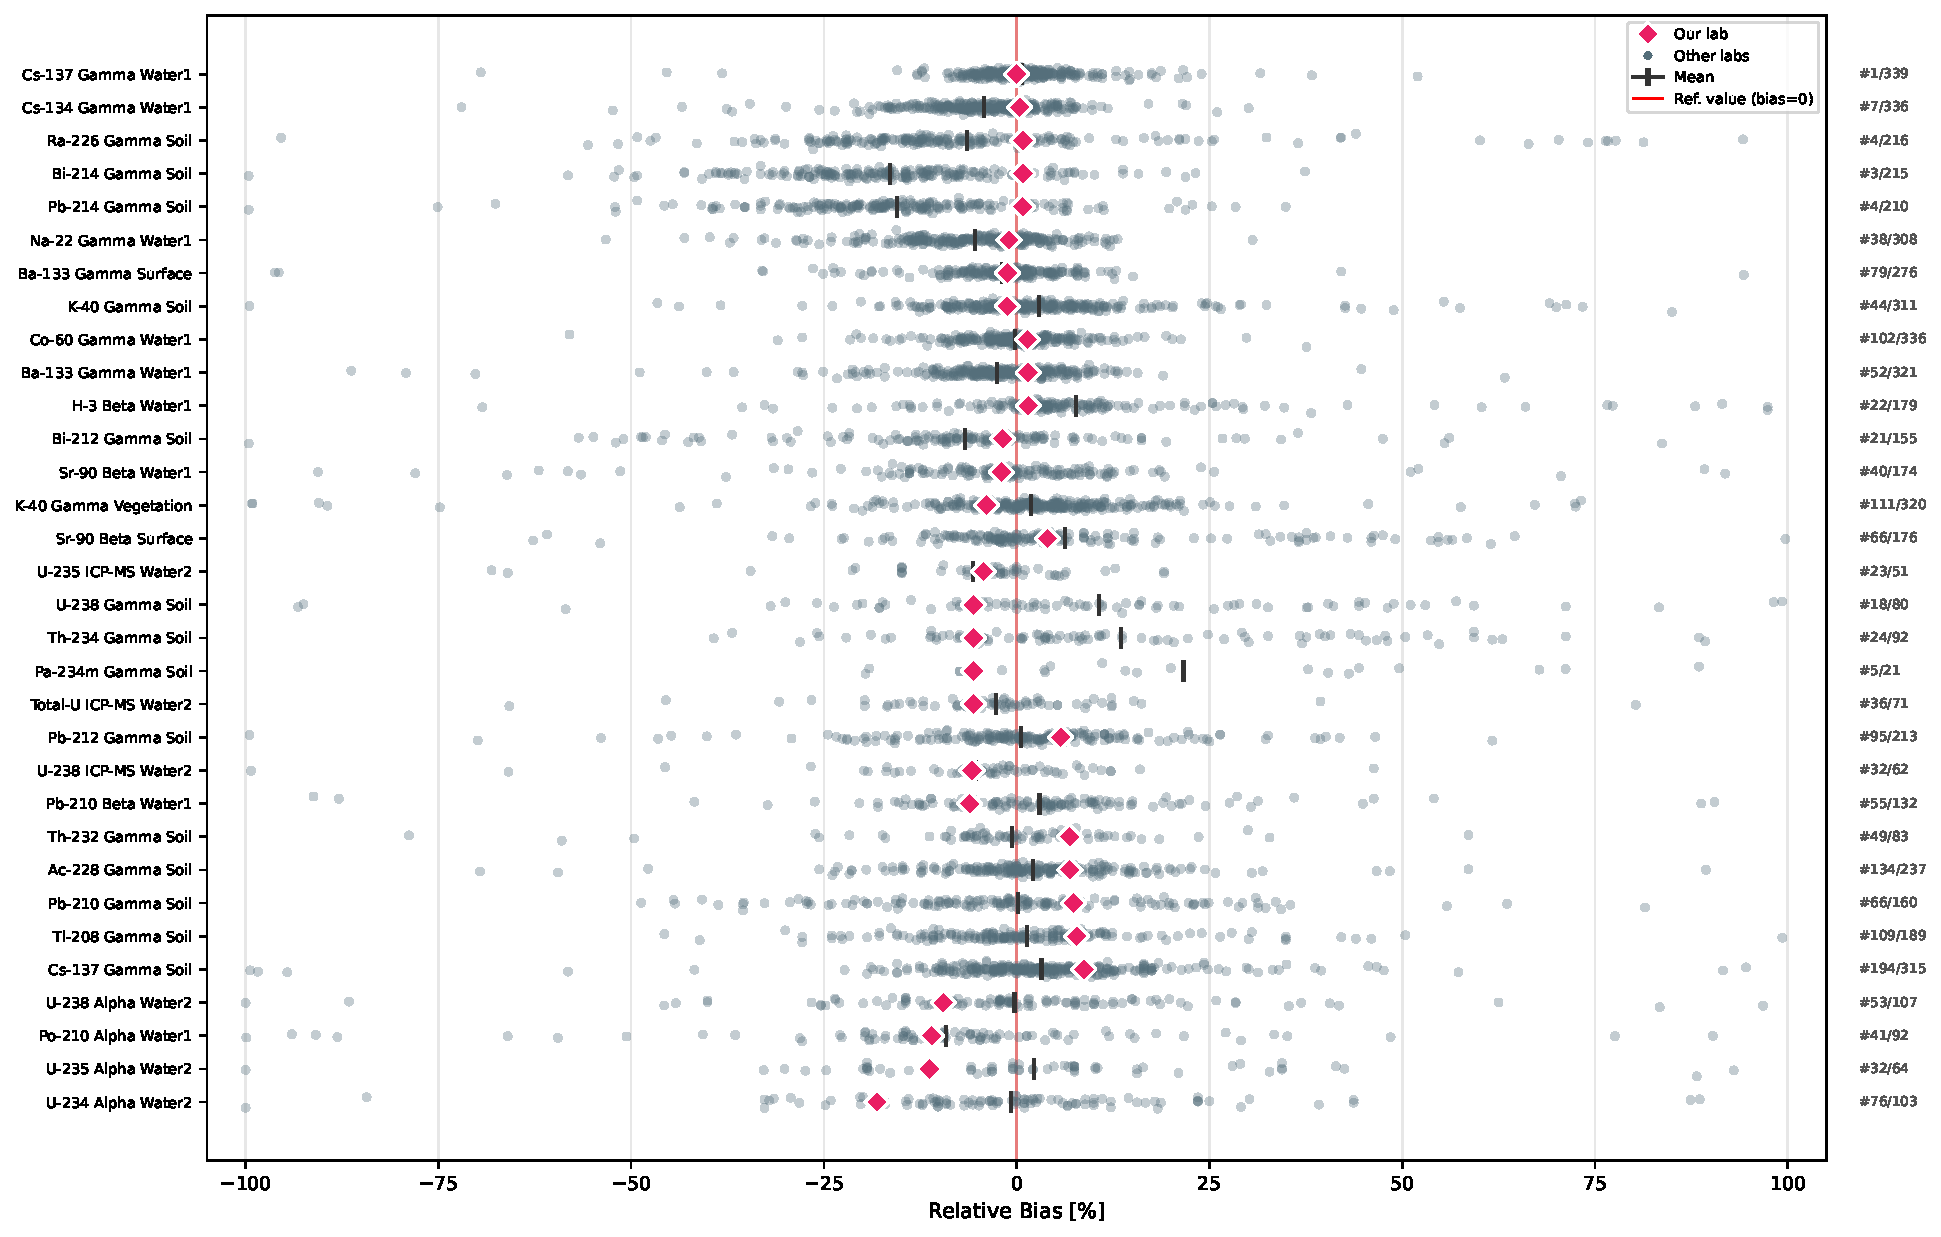
\includegraphics[width=0.98\textwidth]{figures/fig_relative_bias_2025.pdf}
  \caption{Distribution of relative bias per project for the 2025 round. Each row shows one project, sorted by our laboratory's $|\text{bias}|$ (largest at top). Pink diamond = our laboratory; grey dots = other laboratories; tick mark = project mean. Rank annotations (\#rank/total) appear to the right of each row.}
  \label{fig:relative_bias_2025_dist}
\end{figure}

\subsection{Implications and Limitations}

The proposed framework yields actionable insights beyond pass/fail reporting. The RDI enables accuracy tracking year over year, complementing the Z-score evaluation~\cite{thompson2006,zscore}. Difficulty-tier stratification serves as an early warning: the 100\% pass rate through Moderate difficulty and 91.7\% in Hard, both exceeding global averages, indicate genuine robustness rather than avoidance of challenging projects. The bias heatmap identifies specific analytes ($^{210}$Po, uranium isotopes) for targeted method improvement~\cite{iso17025}.

Several limitations should be considered when interpreting these results. (1) The IAEA's anonymized lab-code assignment prevents correlation of performance changes with internal procedural modifications. (2) The difficulty coefficient $D_{j,y}$, as defined with a round-level denominator, conflates intrinsic analytical difficulty with participation breadth; a sensitivity analysis using a project-level denominator ($D^*_{j,y} = 1 - N_{\text{pass}}/N_{\text{total in project}}$) would clarify which projects are genuinely difficult for those who attempt them. (3) The RDI metric evaluates accuracy only and does not penalize underestimated measurement uncertainties. A laboratory that systematically under-reports its uncertainties could achieve a deceptively low RDI. Future work should incorporate an uncertainty-realism metric, such as the $E_n$-number from ISO 13528, to complement the RDI's accuracy focus. (4) Approximately 19\% of the case-study laboratory's measurements (26/135), predominantly gross alpha/beta determinations, lacked reported relative bias values and were excluded from RDI calculations. The impact of this exclusion on the RDI trend is likely modest but cannot be fully quantified without the underlying target values. (5) The framework was demonstrated on a single high-performing laboratory; its diagnostic value for laboratories with weaker or more variable performance profiles, or with fewer annual PT participations, remains to be established. Laboratories with fewer than approximately 10 projects per year may find the RDI dominated by individual outliers. Despite these limitations, the framework is modular and the companion code is publicly available, enabling other laboratories to apply it to their own data and PT providers to evaluate its utility across broader participant cohorts~\cite{povinec2001,alenitz1995}.

% ===================================================================
\section{Conclusions}
% ===================================================================

This study has presented a comprehensive, multi-dimensional analysis of one Chinese radiological laboratory's performance across five consecutive IAEA proficiency test rounds (2021--2025), encompassing 135 individual measurements in 133 radionuclide--matrix combinations. The key findings are:

\begin{enumerate}[nosep,label=(\arabic*)]
  \item The proposed multi-dimensional framework---combining difficulty coefficients, a weighted Result Deviation Index (RDI), tier-stratified pass rates, within-project percentile ranking, and bias heatmaps---provides a richer and more actionable picture of PT performance than the traditional single-project pass/fail report. The framework is modular: each analytical dimension can be adopted independently, and the companion code (available on GitHub) allows other laboratories to apply it to their own PT data with minimal modification.
  \item Applied to the case-study laboratory's 135 measurements across five years, the framework revealed: an overall 98.5\% pass rate with zero ``Not Acceptable'' results; pass rates of 100\% (Very Easy and Easy tiers), 95.0\% (Moderate), and 91.7\% (Hard), substantially exceeding global averages; a weighted RDI of 3.05\% (5-year mean), consistently below the all-laboratory benchmark; and a statistically significant tendency for absolute relative bias to fall below the peer median (Wilcoxon $p < 0.001$, 97/109 projects).
  \item Formal statistical inference provided important nuance to the descriptive findings. Mann--Kendall trend tests over the five annual means did not detect statistically significant temporal trends in difficulty ($p = 0.81$), pass rate ($p = 0.22$), or RDI ($p = 0.086$) at $\alpha = 0.05$. Year-to-year differences in percentile rank distributions were also non-significant (Kruskal--Wallis $p = 0.12$). The observed fluctuations are therefore consistent with random inter-year variation given the limited number of years ($N = 5$); additional years of data will be needed to confirm or refute directional trends.
  \item Within-project relative bias analysis identified $^{137}$Cs, $^{134}$Cs, and decay-chain gamma emitters in soil as areas of outstanding accuracy, and uranium isotopes and $^{210}$Po as areas where method optimization would be most beneficial. The bias heatmap proved particularly effective for revealing subtle but systematic analyte-specific patterns that are invisible in per-project pass/fail reports.
  \item We recommend that laboratories conducting longitudinal PT self-assessment adopt at minimum the RDI metric (for accuracy tracking) and difficulty-tier stratification (to demonstrate competence across the difficulty spectrum). PT providers could facilitate such analyses by publishing project-level difficulty statistics and MARB values for all projects in their summary reports.
\end{enumerate}

The case-study analysis demonstrates that a laboratory can maintain sustained high performance across five PT rounds despite considerable year-to-year variation in project difficulty and a nearly threefold expansion in analytical scope. The framework's value lies not in replacing the IAEA's per-project evaluation, but in complementing it with a longitudinal, multi-dimensional perspective that surfaces patterns invisible to the conventional pass/fail lens.

% ===================================================================
% Acknowledgements
% ===================================================================
\section*{Acknowledgements}
The authors gratefully acknowledge the IAEA Terrestrial Environmental Radiochemistry Centre (TERC) for organizing the proficiency tests and providing detailed evaluation reports. We thank the staff of the Radiation Monitoring Technical Center for their dedicated analytical work over the five-year period.

% ===================================================================
% References
% ===================================================================
\bibliographystyle{unsrturl}
\bibliography{refs}

% ===================================================================
\end{document}
